\documentclass[hidelinks,11pt]{scrreprt}
\usepackage[a4paper,width=150mm,top=25mm,bottom=30mm]{geometry}
\usepackage[utf8]{inputenc}

\usepackage{graphicx}
\graphicspath{{images/}{../images/}}

\usepackage[table]{xcolor}
\usepackage{multirow,tabularx}
\newcolumntype{Y}{>{\centering\arraybackslash}X}

%\usepackage{sectsty}
%\allsectionsfont{\nohang}

\usepackage[titletoc]{appendix}

%\usepackage{titlesec}

\usepackage[numbers]{natbib}
\renewcommand{\refname}{\large References}  % for the article class
\renewcommand{\bibname}{\large References}  % for the report or book class
\def\bibfont{\footnotesize}

% line break in bibliography urls
\usepackage{xurl}

\usepackage{caption}
%\usepackage{tocbibind}

% indent paragraphs
\usepackage{changepage}

\usepackage{mathtools}
\usepackage{amsmath}
\usepackage{amssymb}
\usepackage{amsthm}
\usepackage{color}
\usepackage{float}
\usepackage{bm}
\usepackage{multirow, makecell}
\usepackage{enumitem}
\usepackage{bold-extra}
\usepackage[mathscr]{euscript}

% matrix with labeled rows and columns
\usepackage{kbordermatrix}

\usepackage[linesnumbered,ruled,vlined]{algorithm2e}
\SetKw{Continue}{continue}
\SetKw{Input}{Input:}
\SetKw{Output}{Output:}

%\usepackage{listings}
\usepackage{pythonhighlight}


\DeclareMathOperator{\lca}{lca}
\DeclareMathOperator*{\argmax}{arg\,max}
\DeclareMathOperator*{\argmin}{arg\,min}
\definecolor{darkgrey}{rgb}{0.2,0.2,0.2}
\newcommand{\COMMANDLINE}[1]{\begingroup\par\vspace{3mm}\color{darkgrey}\begin{adjustwidth}{1cm}{1cm}\texttt{#1}\end{adjustwidth}\vspace{3mm}\endgroup}
\newcommand{\TODO}[1]{\begingroup\color{red}#1\endgroup}
\newcommand{\OLD}[1]{\begingroup\tiny   \color{green}#1\endgroup}
\newtheorem{theorem}{Theorem}
\newtheorem{lemma}[theorem]{Lemma}
\newtheorem{corollary}[theorem]{Corollary}
\newtheorem{definition}[theorem]{Definition}
\newtheorem{fact}[theorem]{Observation}
\def\arrowedvec{\mathaccent"017E}
\newcommand{\G}{\arrowedvec{G}}
\newcommand{\unrooted}[1]{\overline{#1}}  
\newcommand{\ROOT}{\circledcirc}
\newcommand{\LEAF}{\odot}
\usepackage{wasysym}
\newcommand{\SPEC}{\newmoon}
\newcommand{\HGT}{\triangle}
\newcommand{\DUPL}{\square}
\newcommand{\child}{\mathsf{child}}
\newcommand{\degree}{\mathsf{deg}}
\newcommand{\parent}{\mathsf{par}}
\newcommand{\bmr}{\mathrel{\bm{\rightarrow}}}
\newcommand{\C}[1]{\mathscr{C}_{#1}}
\newcommand{\AX}[1]{\textnormal{#1}}

% symbol for disjoint union
\makeatletter
\def\moverlay{\mathpalette\mov@rlay}
\def\mov@rlay#1#2{\leavevmode\vtop{%
		\baselineskip\z@skip \lineskiplimit-\maxdimen
		\ialign{\hfil$\m@th#1##$\hfil\cr#2\crcr}}}
\newcommand{\charfusion}[3][\mathord]{
	#1{\ifx#1\mathop\vphantom{#2}\fi
		\mathpalette\mov@rlay{#2\cr#3}
	}
	\ifx#1\mathop\expandafter\displaylimits\fi}
\makeatother
\newcommand{\cupdot}{\charfusion[\mathbin]{\cup}{\cdot}}

% Mark overfull boxes
\overfullrule=1mm

% Hyphenation and line breaks
\hyphenation{du-pli-ca-ti-on}

% contents links etc.
\usepackage{hyperref}
\hypersetup{
	colorlinks=True,
	linkcolor=blue,
	filecolor=magenta,      
	urlcolor=cyan,
	citecolor=black,
}

%\usepackage{setspace}

\begin{document}

\begin{titlepage}
	\begin{center}
		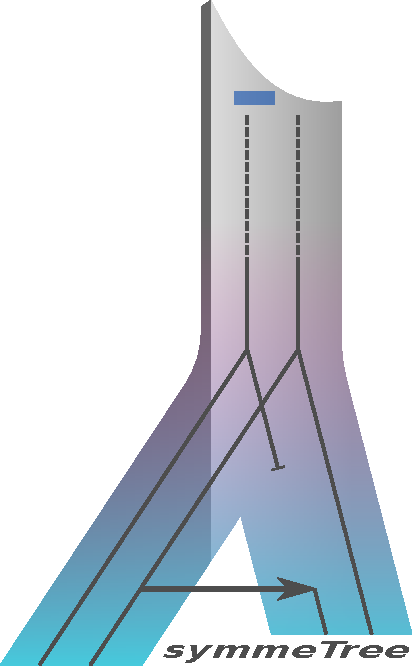
\includegraphics[width=0.4\textwidth]{logo.pdf}
	\end{center}
	\begin{center}
		\vspace*{2cm}
		
		\Huge{\fontfamily{lmtt}
			AsymmeTree User Manual
		}

		\vspace{1.5cm}
		
		\LARGE
		David Schaller\\
		\vspace{1cm}
		\large
		sdavid@bioinf.uni-leipzig.de
		
		\vspace{2cm}
		
	\end{center}
\end{titlepage}

\newpage

\tableofcontents

\chapter{Introduction}

AsymmeTree is an open-source Python library for the simulation and analysis of phylogenetic scenarios.
It includes a simulator for species and gene trees with asymmetric evolution rates, tools for the inference and analysis of phylogenetic best matches \citep{geiss2019a,geiss2020c} (resp. best hits) from known gene trees or evolutionary distances. Moreover, it includes an algorithm to compute supertrees \citep{deng2016} and a method to estimate rooted species trees from an ensemble of orthology/paralogy relations \citep{hellmuth2015}.

The library, and especially the simulator, was primarily designed to be able to validate mathematical concepts and test inference methods for various steps on the way to more realistically available data, i.e., dated gene trees, additive distances of gene sets, noisy distances and finally sequences.
Both nucleotide and amino acid sequence simulation with or without indels are supported. In both cases, several substitution models are available.
Alternatively, third-party software such as \texttt{Pyvolve} \cite{spielman2015} can easily be incorporated into a simulation pipeline based on AsymmeTree.

The software is hosted on \href{https://github.com/david-schaller/AsymmeTree}{GitHub} and also available via The Python Package Index (\href{https://pypi.org/project/asymmetree/}{PyPI}).
Please feel free to report bugs or make suggestions for improvement in the \href{https://github.com/david-schaller/AsymmeTree/issues}{Issues} section of the GitHub repository.

If you use AsymmeTree in your project or code from it, please cite:

\vspace{3mm}
\begin{adjustwidth}{1cm}{1cm}
	Peter F. Stadler, Manuela Gei{\ss}, David Schaller, Alitzel L{\'o}pez S{\'a}nchez, Marcos Gonz{\'a}lez Laffitte, Dulce I. Valdivia, Marc Hellmuth, Maribel Hern{\'a}ndez Rosales (2020). \textbf{From pairs of most similar sequences to phylogenetic best matches.} \textit{Submitted to Algorithms for Molecular Biology.}
\end{adjustwidth}
\vspace{3mm}

This document is split into two parts. Chapter~\ref{sec:manual} is a manual that describes the installation and usage of the package, whereas Chapter~\ref{sec:doc} contains detailed descriptions of the motivation and implementation of the simulator's main components.

\chapter{Manual}\label{sec:manual}

\section{Installation}

AsymmeTree requires Python 3.5 or higher. Python 2 is not supported.

\subsection{Easy Installation with pip}


The \texttt{asymmetree} package is available on The Python Package Index (PyPI):

\COMMANDLINE{pip install asymmetree}

\noindent
For details about how to install Python packages see
\href{https://packaging.python.org/tutorials/installing-packages/}{here}.

\subsection{Installation with the setup file}


Alternatively, you can download or clone the repo, go to the root folder of package and install it using the command:

\COMMANDLINE{python setup.py install}


\subsection{Dependencies}

AssymmeTree has several dependencies (which are installed automatically when using \texttt{pip} or the \texttt{setup.py}):

\begin{itemize}
	\item \href{https://networkx.github.io}{NetworkX}
	\item \href{http://www.scipy.org/install.html}{SciPy and NumPy}
	\item \href{https://matplotlib.org/}{Matplotlib}
\end{itemize}

Furthermore, to use functions involving sequence alignment, the following package(s) must be installed (i.e., they are not installed automatically!):

\begin{itemize}
	\item \href{http://biopython.org/wiki/Download}{Biopython} \citep{cock2009}
\end{itemize}

To use the tree reconstruction method for best match inference and the C++ implementation of the quartet method \citep{stadler2020}, resp., the following software must be installed
(I recommend that you compile these tools on your machine, place the binaries into a persistent location and add this location to your PATH environment variable):

\begin{itemize}
	\item \href{https://birc.au.dk/software/rapidnj/}{RapidNJ} \citep{simonsen2008}
	\item \href{https://github.com/david-schaller/qinfer}{qinfer}
\end{itemize}


\section{Overview}

Table~\ref{tab:module_overview} is an overview over the subpackages and modules that may be relevant for users.

\begin{table}[H]
	\footnotesize
	\setlength{\tabcolsep}{6pt}
	\renewcommand{\arraystretch}{1.4}
	%\renewcommand\tabularxcolumn[1]{m{#1}}
	\begin{tabularx}{\textwidth}{|p{0.26\textwidth}|X|}
		\hline
		\textbf{Packages and Modules} & \textbf{Description} \\
		\hline
		\multicolumn{2}{|l|}{\textbf{\texttt{simulator}}}\\
		\hline
		\texttt{TreeSimulator} & 
		Simulator for dated species trees and dated gene trees, construction of the observable gene tree. \\
		\texttt{TreeImbalancer} & 
		Simulation of evolution rate asymmetries, autocorrelation between ancestors and descendants as well as correlation between genes in the same species. \\
		\texttt{Scenario} & 
		Wrapper class for species and gene tree scenarios, computation of the (R)BMG as well as event counts and some statistics. \\
		\texttt{NoisyMatrix} & 
		Generation of a noisy matrix (\emph{random perturbation} or \emph{wrong topology noise}). \\
		\hline
		\multicolumn{2}{|l|}{\textbf{\texttt{tools}}}\\
		\hline
		\texttt{Tree} & 
		Includes the basic class \texttt{Tree}, provides functions for traversals, Newick parser, etc. \\
		\texttt{PhyloTree} & 
		Includes the class \texttt{PhyloTree} for phylogenetic trees (inherits from \texttt{Tree}), provides a Newick parser, etc. \\
		\texttt{BuildST} & 
		Includes the class \texttt{BuildST} that computes a supertree from a given list of tress (with overlapping labels) \citep{deng2016}. \\
		\hline
		\multicolumn{2}{|l|}{\textbf{\texttt{best\_match\_infer}}}\\
		\hline
		\texttt{TrueBMG} & 
		Computation of the true (R)BMG from a gene tree as well as the true orthology relation. \\
		\texttt{ExtBestHits} & 
		Implementation of the \emph{Extended Best Hits} method, optionally uses \texttt{qinfer}. \\
		\texttt{TreeReconstruction} & 
		Reconstruction of the gene tree with \texttt{RapidNJ} \citep{simonsen2008} and midpoint rooting. \\
		\texttt{Quartets} & 
		Implementation of \emph{Quartet} approach with two different methods for outgroup selection, optionally uses \texttt{qinfer}. \\
		\texttt{LRTConstructor} & 
		Construction of a least resolved tree (LRT) from a BMG via \emph{informative triples}, optionally uses minimal edge cuts. \\
		\hline
		\multicolumn{2}{|l|}{\textbf{\texttt{cograph}}}\\
		\hline
		\texttt{Cograph} & 
		Includes the classes \texttt{Cotree} and \texttt{CotreeNode} as well as a generator for random cotrees/cographs. \\
		\texttt{CographEditor} & 
		Implements a heuristic for cograph editing \citep{crespelle2019}. \\
		\texttt{LinearCographDetector} & 
		Implements an $\mathcal{O}(n+m)$ algorithm for cograph detection \citep{corneil1985}. \\
		\hline
		\multicolumn{2}{|l|}{\textbf{\texttt{paraphylo}}}\\
		\hline
		\texttt{SpeciesTreeFromParalogs} & 
		Species tree reconstruction from orthology/paralogy relations. Heuristic version of \texttt{ParaPhylo} \cite{hellmuth2015}. \\
		\texttt{SpeciesTreeFromPO} & 
		Species tree reconstruction from \texttt{ProteinOrtho} \cite{lechner2011} output. \\
		\hline
		\multicolumn{2}{|l|}{\textbf{\texttt{visualize}}}\\
		\hline
		\texttt{GeneTreeVis} & 
		Visualization of a (simulated) gene tree (of type \texttt{PhyloTree}) \\
		\hline
	\end{tabularx}
	\caption{Overview over the subpackages and modules.}
	\label{tab:module_overview}
\end{table}


\subsection{Tree Data Structures}

The two classes \texttt{Tree} and \texttt{PhyloTree} (inherits from \texttt{Tree}) implement tree data structures which are essential for most of the modules in the package.
The latter contains converters and parsers for the Newick format and a NetworkX graph format.

The vertices of a \texttt{PhyloTree} instance are of type \texttt{PhyloTreeNode} and contain the following attributes:

\vspace{3mm}
\renewcommand{\arraystretch}{1.5}
\begin{tabularx}{0.95\textwidth} { >{\raggedright\arraybackslash}p{3cm} >{\raggedright\arraybackslash}X }
	\texttt{ID} & vertex ID (\texttt{int})\\
	\texttt{label}  & label (\texttt{str}), in gene trees: \texttt{"S"} for speciation, \texttt{"D"} for duplication, \texttt{"H"} for horizontal gene transfer, \texttt{"*"} for loss\\
	\texttt{color} & only gene trees; species in which the gene resides, i.e., ID of some vertex in a species tree, can be of type \texttt{tuple} (edge) for inner and loss vertices\\
	\texttt{tstamp} & time stamp of the event (\texttt{double})\\
	\texttt{dist} & evolutionary distance or divergence time from the parent vertex (\texttt{double})\\
	\texttt{tranferred} & only gene trees; indicates whether the edge from the parent is the transfer edge from an HGT event; \texttt{1} if yes and \texttt{0} otherwise \\
\end{tabularx}
\vspace{3mm}

Both species and gene trees can be converted into Newick format using the function \texttt{to\_newick()} of the \texttt{PhyloTree} class.
In case of a gene tree, the color is represented in brackets, e.g.
\COMMANDLINE{>>> "(3<1>:0.534,2<2>:0.762)S<0>:0.273"}
To suppress this, use \texttt{to\_newick(color=False)}. Likewise, to suppress the distances, you can use \texttt{to\_newick(distance=False)}.
The function \texttt{PhyloTree.parse\_newick()} can handle this customized format as well as the standard Newick format.

If you intend to serialize species or gene trees, I recommend converting them into NetworkX graphs before applying Python's serialization library \texttt{pickle}.
Note that the information about the ID of the root should be saved too:
\vspace{2mm}
\begin{python}
import pickle

# tree is of type PhyloTree
tree_nx, root_id = tree.to_nx()

pickle.dump( (tree_nx, root_id), open("tree.pickle", "wb") )
\end{python}
\vspace{2mm}
To load a tree that was serialized this way use:
\vspace{2mm}
\begin{python}
import pickle
from asymmetree.tools.PhyloTree import PhyloTree

tree_nx, root_id = pickle.load( open("tree.pickle", "rb") )
tree = PhyloTree.parse_nx(tree_nx, root_id)
\end{python}
\vspace{2mm}


\subsection{Simulator for Species and Gene Trees}

The subpackage \texttt{asymmetree.simulator} contains modules for the simulation and manipulation of species trees and gene trees.

\subsubsection{Species trees}

The function \texttt{build\_species\_tree(N)} simulates a dated species tree with \texttt{N} leaves (i.e. recent species) using the `innovation model' described by \citet{keller-schmidt2012}.
The following keyword parameters (with their default value) are available:

\vspace{3mm}
\renewcommand{\arraystretch}{1.5}
\begin{tabularx}{0.95\textwidth} { >{\raggedright\arraybackslash}p{4cm} >{\raggedright\arraybackslash}X }
	\texttt{planted=True} & add a planted root that has the canonical root as its
	single neighbor, this way duplication (and loss) events can occur before the first speciation event in a subsequent gene tree simulation\\
	\texttt{model="innovations"}  & model for the species tree simulation, currently only the `innovation model' is available\\
	\texttt{non\_binary=0.0} & probability that an inner edge is contracted,
	results in a non-binary tree\\
\end{tabularx}
\vspace{3mm}

The time stamps of all vertices are normalized such that the root has time stamp \texttt{1.0} and all leaves have time stamp \texttt{0.0} (see Section~\ref{sec:species_tree}).

Example usage:
\vspace{2mm}
\begin{python}
import asymmetree.simulator.TreeSimulator as ts

S = ts.simulate_species_tree(10, planted=True, non_binary=0.2)
print(S.to_newick())
\end{python}
\vspace{2mm}

\subsubsection{Gene trees}

Dated gene trees are simulated along a given species tree \texttt{S} with a variant of the Gillespie algorithm \citep{gillespie1976}.
To this end, an instance of the class \texttt{GeneTreeSimulator} must be initialized with a species tree of type \texttt{PhyloTree}.
The following parameters are available (keyword arguments are indicated by \texttt{=default}):

\vspace{3mm}
\renewcommand{\arraystretch}{1.5}
\begin{tabularx}{0.95\textwidth} { >{\raggedright\arraybackslash}p{4cm} >{\raggedright\arraybackslash}X }
	\texttt{DLH\_rates} & a \texttt{tuple} of three \texttt{float}s, rates for duplication, loss and HGT events in the Gillespie algorithm\\
	\texttt{dupl\_polytomy=0.0}  & allows non-binary duplication events by specifying
	the lambda parameter for a poisson distribution (copy number = drawn number + 2)\\
\end{tabularx}
\vspace{3mm}

At the moment, loss events in a branch are suppressed whenever this branch is the last survivor in its species branch (by setting the loss rate in the branch to zero).
The behaviour is intended to be made optional in future releases.

Example usage:
\vspace{2mm}
\begin{python}
import asymmetree.simulator.TreeSimulator as ts

# S is a species tree of type PhyloTree
TGT_simulator = ts.GeneTreeSimulator(S)
TGT = TGT_simulator.simulate(DLH_rates)
\end{python}
\vspace{2mm}

The function \texttt{observable\_tree(tree)} returns the observable part of a gene tree, i.e., it copies the tree, removes all branches that lead to loss events only and suppresses all inner nodes with only one child. 
It also removes the planted root.
Example usage:
\vspace{2mm}
\begin{python}
# observable gene tree
OGT = ts.observable_tree(TGT)
\end{python}
\vspace{2mm}


\subsubsection{Gene tree imbalancing}

The module \texttt{TreeImbalancer} contains a function to model realistic (asymmetric) evolution rates for a given gene tree (see Section~\ref{sec:imbalancing_implementation}).
Moreover, correlation in the evolution rate between genes of the same (and closely related) species is introduced (autocorrelation).
The function \texttt{imbalance\_tree(T, S)} takes a gene tree \texttt{T} and the \textbf{corresponding} species tree \texttt{S} as input and manipulated the branch length of the species tree.
The following keyword parameters (with their default values) are available:

\vspace{3mm}
\renewcommand{\arraystretch}{1.5}
\begin{tabularx}{0.95\textwidth} { >{\raggedright\arraybackslash}p{5.6cm} >{\raggedright\arraybackslash}X }
	\texttt{baseline\_rate=1.0} & starting value for the substitution rate (per time unit) and expected value for conserved genes\\
	\texttt{autocorrelation\_variance=0.0}  & variance factor for a lognormal distribution that controls autocorrelation between genes of the same (and closely related) species, the higher the lower the auto\-corre\-la\-tion\\
	\texttt{gamma\_param=(0.5, 1.0, 2.2)}  & parameter the for Gamma distribution (\texttt{a, loc, scale}) from which rate factors for divergent are drawn, the default values are chosen to fit observed asymmetries between paralogs in yeast data \citep{byrne2007}\\
	\texttt{weights=(1, 1, 1)}  & weights for choice between conservation,
	subfunctionalization and neofunctionalization after a duplication event\\
	\texttt{inplace=True}  & manipulate edge lengths (\texttt{dist}) of the gene tree in-place, otherwise copy the tree\\
\end{tabularx}
\vspace{3mm}

In is recommended to apply the imbalancing to the true gene tree that still contains loss events.
Example usage:
\vspace{2mm}
\begin{python}
import asymmetree.simulator.TreeSimulator as ts
import asymmetree.simulator.TreeImbalancer as tm

S = ts.simulate_species_tree(10)

# true gene tree (with losses)
TGT_simulator = ts.GeneTreeSimulator(S)
TGT = TGT_simulator.simulate( (0.5, 0.5, 0.5) )    # event rates D, L, H

# imbalancing
TGT = tm.imbalance_tree(TGT, S, baseline_rate=1,
                        autocorrelation_variance=0.2,
                        gamma_param=(0.5, 1.0, 2.2),
                        weights=(1, 1, 1))

# observable gene tree
OGT = ts.observable_tree(TGT)
\end{python}
\vspace{2mm}


\subsubsection{Distance matrix and noise simulation}

The additive distance from an \textbf{observable} gene tree can be computed using the function \texttt{distance\_matrix()} of a \texttt{PhyloTree} instance.
It returns a tuple containing a list of leaves in the tree (specifying the indexing) and the distance matrix as a 2-dimensional \texttt{numpy} array.

\vspace{2mm}
\begin{python}
# T is an observable gene tree
leaves, D = T.distance_matrix()
leaf_index_dict = {leaf: i for i, leaf in leaves}
\end{python}
\vspace{2mm}

In the next step, noise can be introduced into a distance matrix using the \texttt{NoisyMatrix} module.
Random noise can be simulated with the function \texttt{noisy\_matrix(orig\_matrix, sd)}.
The following parameters are available (keyword arguments are indicated by their default value):

\vspace{3mm}
\renewcommand{\arraystretch}{1.5}
\begin{tabularx}{0.95\textwidth} { >{\raggedright\arraybackslash}p{4.5cm} >{\raggedright\arraybackslash}X }
	\texttt{orig\_matrix} & original matrix to be disturbed\\
	\texttt{sd}  & standard deviation of a normal distribution with mean 1 from which noise factors are drawn\\
	\texttt{metric\_repair="reject"}  & method to ensure that the resulting distance matrix is still a metric, available are \texttt{"reject"}, \texttt{"DOMR"} and \texttt{"general"} (see Section~\ref{sec:measurement_noise})\\
\end{tabularx}
\vspace{3mm}

Alternatively, the function \texttt{convex\_linear\_comb(D1, D2)} can be used to simulate systematically biased noise by computing a linear convex combination with a disturbance matrix.
The function thus takes two distance matrices (\texttt{numpy} arrays) not necessarily of the same size as input and disturbs them with one another.
The contribution of the respective disturbance matrix is controlled by the keyword parameter \texttt{alpha} (default is \texttt{0.5}).
If the keyword parameter \texttt{first\_only} is specified as \texttt{True}, only the first disturbed matrix is returned.
Otherwise both are returned in a tuple.


\subsection{Best Match Inference}

Phylogenetic best matches of a gene $x$ of species $X$ are defined as those genes $y$ of another species $Y\ne X$ that share the lowest common ancestor with $x$ in the gene tree among all genes in that species \citep{geiss2019a,geiss2020b,geiss2020c}, see also Section~\ref{sec:homology_and_bm}.
In contrast, two genes are orthologs if their last common ancestor was a speciation event.
Orthology and reciprocal best matches are closely related \citep{geiss2020c}.

The subpackage \texttt{asymmetree.best\_matches} contains functions to compute both relations from a given gene tree or to estimate them from distance data on a set of genes \citep{stadler2020}.

If the true (observable) gene tree is known (as e.g.\ the case in simulations), best matches and orthologs can be computed using the module \texttt{TrueBMG}.
The functions \texttt{best\_match\_ graphs(tree)} and \texttt{true\_orthology\_graph(tree)} return the respective graph representation as NetworkX (di)graphs:

\vspace{2mm}
\begin{python}
from asymmetree.best_matches.TrueBMG import true_orthology_graph, best_match_graphs

# T is an observable gene tree
orthology_graph = true_orthology_graph(T)
BMG, RBMG = best_match_graphs(T)    # Best Match Graph and Reciprocal Best Match Graph as a tuple
\end{python}
\vspace{2mm}

If only distance data is available, best matches have to be estimated.
AsymmeTree currently implements three different methods that are described by \citet{stadler2020}:
\begin{itemize}
	\item Extended Best Hits (module \texttt{ExtBestHits})
	\item Neighborjoining and midpoint rooting (module \texttt{TreeReconstruction}, requires the installation and accessibility of \texttt{RapidNJ} \citep{simonsen2008})
	\item Quartet method (module \texttt{Quartets}, Python implementation and wrapper for the C++ tool \texttt{qinfer})
\end{itemize}

Please see the file \texttt{examples/best\_match\_infer.py} in the GitHub repo for an example usage of these modules following the simulation of gene tree scenarios.



\subsection{Supertree Computation}

The module \texttt{BuildST} contains an implementation of the BuildST algorithm described by \citet{deng2016} to compute a supertree from a given list of tree based on the leaf labels.
The algorithm uses the dynamic graph data structure described by \citet{henzinger1995} and \citet{holm2001}.
The latter can also be used separately (see module \texttt{asymmetree.tools.hdtgraph.DynamicGraph})

The class \texttt{BuildST} is initialized with a list of trees that are of type \texttt{Tree} (thus also \texttt{PhyloTree} is allowed).
The method \texttt{run()} then return a supertree if the trees in the list are compatible \emph{and} they overlap in their sets of leaf labels.
More precisely, the graph on the set of input trees in which two trees are connected by an edge if and only if they have at least one leaf label in common must be connected.

Example usage:

\vspace{2mm}
\begin{python}
from asymmetree.tools.BuildST import BuildST

# tree_list is a list of Tree instances
st_builder = BuildST(tree_list)
supertree = st_builder.run()

if supertree:
	print(supertree.to_newick())
else:
	print("Could not build a supertree!")
\end{python}
\vspace{2mm}


\subsection{Cograph Editing and ParaPhylo}

The subpackages \texttt{asymmetree.cograph} and \texttt{asymmetree.proteinortho} contain heuristics for cograph editing and a method to compute rooted species tree from orthology/paralogy relations.
The latter is a reimplementation of \href{http://pacosy.informatik.uni-leipzig.de/208-0-ParaPhylo.html}{ParaPhylo} \citep{hellmuth2015} which uses heuristics for the NP-hard steps instead of exact ILP solutions.
For cograph editing, the $\mathcal{O}(n^2)$ algorithm (where $n$ is the number of vertices in a connected graph) by \citet{crespelle2019} is applied.
For the Maximum Consistent Triple Set problem, tree different heuristics are available:
\begin{itemize}
	\item \texttt{BPMF}: Best-Pair-Merge-First \citep{wu2004} (modified for weighted triples)
	\item \texttt{MINCUT}: Aho's \texttt{BUILD} with weighted MinCut \citep{aho1981,byrka2010}
	\item \texttt{GREEDY}: a greedy approch based on Aho's \texttt{BUILD}
\end{itemize}

The class \texttt{TreeReconstructor} in the module \texttt{SpeciesTreeFromParalogs} computes a species tree after it is provides with one or more NetworkX graphs that represent (estimated) orthology relations.
To this end, the nodes in these graph must have a \texttt{"color"} attribute, since these will be the leaf labels in the reconstructed species tree.
Example usage:
\begin{python}
from asymmetree.paraphylo.SpeciesTreeFromParalogs import TreeReconstructor

tree_reconstr = TreeReconstructor()

# ortho_relations is a list of orthology relations
for graph in ortho_relations:
    tree_reconstr.add_ortho_graph(graph)
    
# finally the tree can be computed
S_estimate = tr.build_species_tree(mode="BPMF")
print(S_estimate.to_newick())
\end{python}
\vspace{2mm}

The module \texttt{SpeciesTreeFromPO} contains functions to estimate a species tree from a \texttt{ProteinOrtho} output file. For example, the function \texttt{reconstruct\_from\_PO(filename, triple\_mode="BPMF")} takes the filename to the \texttt{ProteinOrtho} output file and optionally the triple heuristic as input, and returns a tuple consisting of the estimated species tree (\texttt{PhyloTree}) and a Newick representation (\texttt{str}) containing support values for the inner nodes.


\chapter{Documentation of the Gene Family Simulator}\label{sec:doc}

A first version of this simulator for species trees and gene families was part of my Master's thesis \citep{schaller2019} and has been used by \citet{stadler2020}.
Parts of the following sections including some images have been reused from my thesis.

\section{Mathematical Preliminaries}
\label{sec:prelim}

\subsection{Graph and Tree Notation}
In this section, a very short introduction into the field of graph theory is given with a focus on the concepts that will be relevant in the subsequent sections.
For standard textbooks see e.g.\ \cite{diestel2017} and \citet{semple2003} from which definitions in the following were taken. The notation concerning trees follows the one used by \citet{geiss2019a}.

\begin{definition}[(Di-)Graph]
	A \emph{graph} is a pair $G=(V,E)$ of sets such that $E \subseteq [V]^2$, i.e., the elements of $E$ are 2-element subsets of $V$. The elements in $V$ are called vertices or nodes and the elements in $E$ are called edges. Here, an (undirected) edge $e$ between vertices $x$ and $y$ is written as $xy$.
	
	A \emph{directed graph} (or \emph{digraph}) is s graph that assigns to every edge an initial and terminal vertex. In this case, an edge $e$ is written as $(x,y)$ if $x$ is the initial, and $y$ is the terminal vertex of edge $e$.
\end{definition}

As usual, it is often written $V(G)\coloneqq V$ and $E(G)\coloneqq E$ for the sets of vertices and edges of a graph $G=(V,E)$ in order to express affiliation. Two vertices $x$ and $y$ are \emph{adjacent} if $xy\in E(G)$ [or $(x,y)\in E(G)$, respectively]. The \emph{degree} of a vertex $x$ is the number of adjacent vertices and denoted by $\degree(x)$.

The notation $G[x_1,...,x_k]$ refers to an induced subgraph $G'$ of a graph $G$ on the set $V(G')=\{x_1,...,x_k\}\subseteq V(G)$. Induced subgraphs are defined in the usual sense, i.e., $xy\in E(G')$ [or $(x,y)\in E(G')$ if $G$ is directed] if and only if $xy\in E(G)$ [$(x,y)\in E(G)$] and $x,y\in V(G')$.

An undirected graph $G=(V,E)$ is called \textit{connected} if any two vertices $x,y \in V(G)$ are linked by a path in $G$, i.e., there is a path $x=x_1-x_2-...-x_k=y$ such that $x_ix_{i+1} \in E(G)$ for all $1 \le i < k$.
A maximal connected subgraph of $G$ is called a \textit{connected component} of $G$. In case of a directed graph $\G$, a subgraph $\G^*$ of $\G$ is called a \textit{strongly connected component} if for any two vertices $x$ and $y$ there is directed path $x=x_1 \rightarrow x_2\rightarrow ...\rightarrow x_k=y$ such that $(x_i,x_{i+1}) \in E(\G)$ for all $1 \le i < k$ and vice versa. Furthermore, $\G^*$ must be maximal in that sense.

Given a non-empty set of colors $\mathcal{C}$, a \emph{proper vertex coloring} of a (di-)graph $G$ is a map $\sigma \colon V(T) \to \mathcal{C}$ such that $xy \in E(G) \implies \sigma(x) \ne \sigma(y)$. In other words, two adjacent vertices must not have the same color.

\begin{definition}[Rooted tree]
	A graph $T=(V,E)$ is a \emph{tree} if it is connected and acyclic. A \emph{rooted tree} is a tree $T$ with a special node $\rho$ called the \emph{root}. As a consequence of this, a partial order $\preceq_T$ on the vertex set $V(T)$ can be defined where $v \preceq_T u$ if $u$ lies on the (unique) path from $\rho$ to $v$.
\end{definition}

A vertex $u$ is called an \textit{ancestor} of $v$ in $T$ if $v \preceq_T u$, whereas $v$ is a descendant of $u$ in this case. If furthermore $uv \in T$, then $u$ is the parent of $v$, and $v$ is a child of $u$. The set of all children of a vertex $u$ is denoted by $\child(u)$. Likewise, $\parent(v)$ refers to the unique parent of a vertex $v$. It is set $\parent(v)=\emptyset$ if $v$ has no parent, i.e., $v$ is the root.

The set of all outer vertices $v \in V(T)$ (i.e., for which $\deg(v)=1$) is called the \textit{leaf set} of $T$ and denoted by $L(T)$. Hence, the leafs $L(T)$ are the minima and $\rho$ is the unique maximum w.r.t.\ $\preceq_T$.
The set of inner vertices $V(T)\setminus L(T)$ is denoted by $V^0(T)$, and a subtree of $T$ which is rooted at a vertex $u \in V^0(T)$ and contains all nodes and edges below $u$ by $T(u)$. Likewise, $L(T(u))$ is the set of leaves under $u$.

A \emph{leaf coloring} is a surjective map $\sigma\colon L(T) \to \mathcal{C}$ that assigns a color to the set of leaves of a tree.
Given such a map, $L[r]$ refers to the set of leaves with color $r\in\mathcal{C}$; more formally $L[r]\coloneqq \{x\in L(T)\,|\,\sigma(x)=r\}$.

The last common ancestor $\lca(A)$ of a subset $A \subseteq V(T)$ is the smallest vertex $v \in V(T)$ (w.r.t.\ $\preceq_T$) such that $x \preceq_T v$ for all $x \in A$. For easier notation, let $\lca(x,y) \coloneqq \lca(\{x,y\})$.

% ($T' \le T$)
A tree $T$ \textit{displays} another tree $T'$ if $T'$ can be obtained from a subtree of $T$ by contraction of edges (in the usual sense).
If not stated otherwise, the displayed tree for a restricted set of leaves $L'$ of $T$ means the tree that is obtained by subsequently  removing all $v \in V(T) \setminus L'$ with $|\child(v)| = 0$ (including their incident edges) and contracting vertices $v \in V(T)$ with $|\child(v)| = 1$ and their two incident edges into a single edge. \emph{Rooted triples} are a special kind of displayed trees. A rooted triple $xy|z$ is a rooted tree on three leaves $x,y,z$ such that the path from $x$ to $y$ and the path from $z$ to the root do not intersect.
A rooted triple is called consistent with a tree $T$ if $x,y,z \in L(T)$ and $\lca(x,y) \prec_T \lca(x,z) = \lca(y,z)$.

The term rooted triple is closely related to the definition of outgroups:

\begin{definition}[Outgroup]
	\label{def:outgroup}
	A leaf $z\in L(T)$ is called an \emph{outgroup} w.r.t.\ a set $X \subset L(T)$ if $\lca(X) \prec \lca(X \cup \{z\})$.
\end{definition}

In particular, $T$ displays the rooted triple $x'x''|z$ for all distinct $x',x''\in X$ and $z \in L(T) \setminus L(T(\lca(X)))$.

Finally, a tree $T$ (and a graph in general) can be endowed with a map that assigns weights to its edges. In the case of positive weights, these can be interpreted as the lengths of the edges and represented by a weight function $\ell\colon E(T) \to \mathbb{R}^+$.

% Phylogentic trees
% reconciliation map, event labeling
\subsection{Phylogenetic Trees}
\label{sec:phylogenetic_trees}

This section describes the properties and the associated maps of phylogenetic trees, i.e., graph models of evolutionary histories of either species or genes.

\begin{definition}[Phylogenetic tree {\citep[cf.][]{hernandez-rosales2012,geiss2020c}}]
	An unrooted tree $\unrooted{T}$ is a \emph{phylogenetic tree} if every inner vertex $v \in V^0(\unrooted{T})$ has a degree of at least 3. A rooted tree $T$ is a \emph{phylogenetic tree} if every $v \in V^0(T)$ has at least 2 children.
	$\unrooted{T}$ and $T$ are called \emph{fully-resolved} if the respective equalities hold, i.e., $\degree(v)=3$ for every $v \in V^0(\unrooted{T})$ or $|\child(v)|=2$ for every $v \in V^0(T)$, respectively.\\
	A \emph{planted} phylogenetic tree $T$ is a rooted phylogenetic tree with a special vertex $0_T$, called the \emph{planted root}, that has a single child $\rho_T$ such that $T(\rho_T)$ is a phylogenetic tree.
\end{definition}

The purpose of this definition is to avoid vertices of degree 2 (possibly with exception of the root). Such vertices would lack a justification by an evolutionary event that could be reconstructed from observable data with suitable methods. In contrast, a vertex that is not fully-resolved can be interpreted as missing information about the exact local topology in most cases. The planted edge $0_T\rho_T$ is useful in the wake of modeling events that predate the first branching event. This becomes especially relevant for the reconciliation of gene trees with the underlying history of the corresponding species, since, e.g., duplication events can occur before the first speciation.

Exact methods for phylogenetic reconstruction cannot per se determine the location of the root. Hence, it is often necessary to consider unrooted trees. An unrooted version $\unrooted{T}$ of a rooted tree $T$ with distance function $\ell$ can be obtained by the following two operations \citep{stadler2020}:
\begin{enumerate}[label=(\roman*), itemsep=0.2cm, topsep=0.2cm, parsep=0cm]
	\item Omit the planted root $0_T$ and its incident edge.
	\item In case the root $\rho_T$ has exactly two children $u_1$ and $u_2$, replace the path \mbox{$u_1-\rho_T-u_2$} by a single edge $u_1u_2$ with length $\ell(u_1u_2) \coloneqq \ell(\rho_Tu_1) + \ell(\rho_Tu_2)$.
\end{enumerate}
The weight function $\ell$ is the same for all other edges. However, note that the ancestor order $\preceq_T$ must be dropped.

As already mentioned, phylogenetic trees can either be species trees, that represent the relationship and branching history of different taxa, or gene trees, which constitute the history of a gene family. In the latter case, duplication and HGT events cause additional branching, whereas losses terminate existing branches.
Since all members of a gene family reside in some species, there exists an embedding of a gene tree $T$ into the corresponding species tree $S$.

In case of a gene tree $T$ on a set of extant genes $L(T)$, the knowledge about which genes reside in which species is represented by a leaf coloring $\sigma\colon L(T) \to L(S)$. Therefore, the color and species of a leaf $v\in L(T)$ will be used as synonymous terms. The rest of the embedding can be formalized by a reconciliation map:

\begin{definition}[Reconciliation Map {\citep[cf.][]{geiss2020c,stadler2020}}]
	\label{def:reconc_map}
	Let $S=(W,F)$ and $T=(V,E)$ be two planted phylogenetic trees and let $\sigma\colon L(T) \to L(S)$ be a surjective map. A reconciliation from $(T,\sigma)$ to $S$ is a map $\mu\colon V \to W \cup F$ satisfying
	\begin{enumerate}[label=\emph{(R\arabic*)}, ref=\emph{(R\arabic*)}, itemsep=0.2cm, topsep=0.2cm, parsep=0cm]
		\setcounter{enumi}{-1}
		\item \emph{Root Constraint.} $\mu(x) = 0_S$ if and only if $x=0_T$.
		\item \emph{Leaf Constraint.} If $x \in L(T)$, then $\mu(x)=\sigma(x)$.
		\item \emph{Ancestor Preservation.} If $x \prec_T y$, then $\mu(x) \preceq_S \mu(y)$.
		\item \emph{Speciation Constraints.} Suppose $\mu(x) \in W^0$.
		\begin{enumerate}[label=(\roman*), itemsep=0.2cm, topsep=0.2cm, parsep=0cm]
			\item $\mu(x)=\lca_S(\mu(v'),\mu(v''))$ for at least two distinct children $v',v''$ of $x$ in $T$.
			\item $\mu(v')$ and $\mu(v'')$ are incomparable in $S$ for any two distinct children $v'$ and $v''$ of $x$ in $T$.
		\end{enumerate}
		\item \emph{Speciation Constraint II.} If $\mu(\lca_T(x,y))=\mu(\lca_T(x,z))\in V^0(S)$, then \newline $\lca_S(\sigma(x),\sigma(y))=\lca_S(\sigma(x),\sigma(z))$ for all distinct leaves $x,y,z\in L(T)$.
	\end{enumerate}
\end{definition}

Axioms \AX{(R0)} to \AX{(R4)} hold for gene family histories that do not include horizontal gene transfer events.
The first two axioms ensure that the root and leaves of $T$ also map to the root and leaves in the species tree $S$, respectively. Note that the \emph{Leaf Constraint} thereby implicitly prohibits loss leaves since they could not be mapped to an extant species. Thus, both $\sigma$ and $\mu$ would be undefined for such kind of leaves.
The \emph{Ancestor Preservation} constraint forbids that a descendant $x$ of some vertex $y$ in $T$ is mapped above $\mu(y)$ in $S$ which avoids time traveling of a gene into an ancestor species.
The two constraints in \AX{(R3)} refer to restrictions for (observable) speciation events in the gene tree. In particular, \AX{(R3 ii)} states that any two children $v'$ and $v''$ of such a vertex are not only incomparable in $T$ but also in $S$, i.e., $\mu(v')$ and $\mu(v'')$ are incomparable w.r.t.\ $\preceq_S$. This corresponds to a separated evolution of the gene family in the descending branches of a speciation event.
Finally, axiom~\AX{(R4)} has been introduced only recently by \citet{stadler2020}. It forbids to map two vertices $v_1,v_2\in V^0(T)$ that represent distinct speciation events to the same vertex in $S$. This avoids ambiguous interpretations of single vertices as multiple events.

In case of the occurrence of HGT events, the axiom system has to be modified \citep{geiss2020c}. First, a weaker version of axiom \AX{(R2)} is satisfied:
\emph{\begin{enumerate}[label=\emph{(R\arabic**)}, ref=\emph{(R\arabic*)}, itemsep=0.2cm, topsep=0.2cm, parsep=0cm, leftmargin=*]
		\setcounter{enumi}{1}
		\item \emph{Weak Ancestor Preservation.} If $x \prec_T y$, then either $\mu(x) \preceq_S \mu(y)$ or $\mu(x)$ and $\mu(y)$ are incomparable w.r.t.\ $\preceq_S$.
\end{enumerate}}
\noindent Moreover, two additional axioms are necessary:
\emph{\begin{enumerate}[label=\emph{(R\arabic*)}, ref=\emph{(R\arabic*)}, itemsep=0.2cm, topsep=0.2cm, parsep=0cm, leftmargin=*]
		\setcounter{enumi}{2}
		\item
		\begin{enumerate}[label=(\roman*), itemsep=0.2cm, topsep=0.2cm, parsep=0cm, leftmargin=*]
			\setcounter{enumii}{2}
			\item \emph{(Addition to the Speciation Constraints.)} Suppose $\mu(x) \in W^0$. If $\mu(x)\in W^0$, then $\mu(v) \preceq_S \mu(x)$ for all $v \in \child(x)$.
		\end{enumerate}
		\setcounter{enumi}{4}
		\item \emph{HGT Constraint.} If $x$ has a child $y$ such that $\mu(x)$ and $\mu(y)$ are incomparable, then $x$ also has a child $y'$ with $\mu(y') \preceq_S \mu(x)$.
\end{enumerate}}
\noindent This extended axiom system is a valid generalization in most cases. However, it fails in some scenarios, e.g., \AX{(R3 ii)} may not hold if an HGT event has no surviving members in the non-transferred branch \citep[cf.][Section 7.3]{geiss2020c}.

An event labeling that is based on the reconciliation map is defined as follows:

\begin{definition}[Event Labeling {\citep[][Def. 3 with HGT]{geiss2020c}}]
	\label{def:event_labeling}
	Given a reconciliation map $\mu$ from $(T,\sigma)$ to $S$, the \emph{event labeling on $T$ (determined by $\mu$)} is the map $t\colon V(T) \to \{ \ROOT,\LEAF,\SPEC,\DUPL,\HGT \}$ given by:
	\begin{equation*}
	t(u) = \left\{
	\begin{array}{ll}
	\ROOT \quad \textrm{if } u=0_T \textrm{, i.e., } \mu(u)=0_S\, \textrm{(root)}\\
	\LEAF \quad \textrm{if } u \in L(T) \textrm{, i.e., } \mu(u) \in L(S)\, \textrm{(leaf)}\\
	\SPEC \quad \textrm{if } \mu(u) \in V^0(S)\, \textrm{(speciation)}\\
	\DUPL \quad \textrm{if } \mu(u) \in E(S)\,\textrm{, } u\,\textrm{and } v\,\textrm{are comparable for all } v \in \child(u)\, \textrm{(dupl.)}\\
	\HGT \quad \textrm{if } u\, \textrm{has a child } v\, \textrm{such that } \mu(u)\, \textrm{and } \mu(v)\, \textrm{are incomparable (HGT)}
	\end{array}
	\right.
	\end{equation*}
\end{definition}

Note that Definition \ref{def:event_labeling} does not capture loss events. As they have shown to be an important cause of problems for inference methods, trees that additionally contain all branches leading to loss events will often be considered. Such complete gene family histories will be referred to as \emph{extended gene trees}. Loss events will be indicated by $\dashv$ (or an asterisk $*$ in the implementation, reps.), whilst the symbols of the event labeling are used for all other event types. In this context, phylogenetic trees in the usual sense correspond to the observable part of the complete gene trees. Observable gene trees are easily constructed from the latter:
\begin{enumerate}[label=(\roman*), itemsep=0.2cm, topsep=0.2cm, parsep=0cm]
	\item Remove all branches leading to loss events only.
	\item Subsequently, contract all nodes of degree 2 (except the root) and the adjacent edges into a single edge.
\end{enumerate}
In ambiguous cases, the observable gene tree will sometimes be denoted by $T_\textrm{obs}$.
An example of an (extended) gene tree $T$ embedding is shown in Figure~\ref{fig:embedded_tree}. It contains the different event types including losses.

\vspace{5mm}
\begin{figure}[ht]
	\begin{center}     
		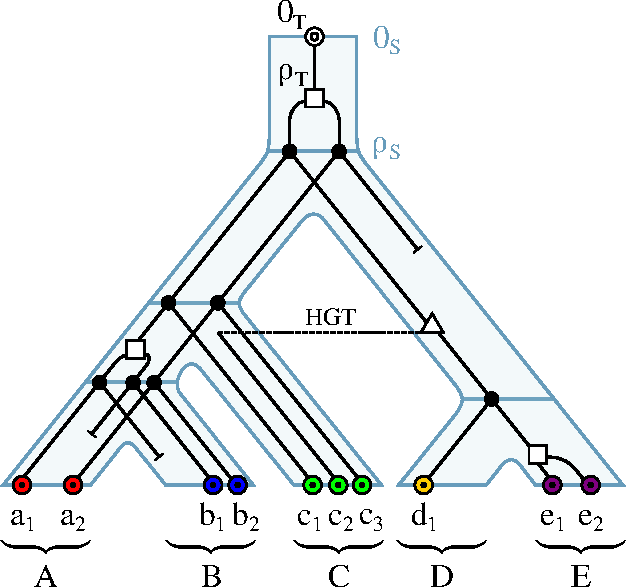
\includegraphics[width=0.55\columnwidth]{embedded_tree.pdf}
	\end{center}
	\caption[Embedding of an extended gene tree into the corresponding species tree]{Embedding of an extended gene tree into the corresponding species tree. The species tree $S$ on the set of extant species $\{A,B,C,D,E\}$ is shown in light blue. The gene family history includes speciation ($\SPEC$), duplication ($\DUPL$), HGT ($\HGT$) and loss ($\dashv$) events. The colors of the non-loss leaves ($\LEAF$) constitute known information about the extant genes, i.e., the species in which they reside.}
	\label{fig:embedded_tree}
\end{figure}

Note that the root $\rho_T$ is not a speciation event but a duplication in the example. Since it will be useful later, the following special type of duplication events is introduced:

\begin{definition}
	\label{def:ancient_dupl}
	A duplication event $v\in V^0(T)$ is called \emph{ancient} if $v$ is
	mapped to the edge $0_S\rho_S$ under the reconciliation map $\mu$.
\end{definition}
It will sometimes be necessary to consider duplication events that predate the last common ancestor of a subset $L' \subseteq L(T)$. Ancient duplications w.r.t.\ $u=\lca_T(L')$ are defined by applying Definition \ref{def:ancient_dupl} to the subtree $T(u)$ where the unique path between $0_T$ and $u$ is contracted into a planted edge for $T(u)$.

Since all vertices in phylogenetic trees represent evolutionary events, it is useful to have a dating function $\tau$ that assigns a time point to every vertex. Following the conventions e.g.\ used by \citet{bocker1998}, these time points will be normalized such that $\tau(0_S)=1$ and $\tau(x)=0$ for all $x \in L(S)$. In case the tree is not planted, $\tau(\rho_T)$ is set to 1. Hence, the dating function maps to the unit interval: $\tau\colon V(T) \to [0,1]$. 



\subsection{Metrics and Ultrametrics}
\label{sec:metrics}

Both the dating function $\tau\colon V(T) \to [0,1]$ and the weight function $\ell\colon E(T) \to \mathbb{R}^+$ can be used to define a distance function on the set of vertices of a tree. Since the dating function assigns time points to the vertices of $T$, the time difference between two vertices $x$ and $y$ (that are comparable in $T$) can be interpreted as the time of divergence that lies between them. In general, the \emph{divergence time} $d_{\tau}$ between two arbitrary nodes $x,y \in V(T)$ is given by
\begin{equation}
d_\tau(x,y) = \sum_{uv \in P} |\tau(u) -\tau(v)|
\end{equation}
where $P$ is the unique path between $x$ and $y$. In contrast, the weighting function $\ell$ can be used to model different aspects of the evolutionary history. In particular, the weights can represent the dissimilarity or evolutionary distance of adjacent vertices in a gene tree $T$.
Thus, the distance that is given by the sum of all edge weights on the unique path $P$ between two vertices $x,y \in V(T)$
\begin{equation}
\label{eq:distance_function}
d(x,y) = \sum_{e \in P} \ell(e)
\end{equation}
corresponds to the \emph{evolutionary distance} between $x$ and $y$.

The set of vertices $V(T)$ together with one of the two distance functions $d_\tau$ or $d$ forms a \emph{metric space}. A metric is defined as follows:

\begin{definition}[Metric \& Ultrametric]
	\label{def:metric}
	A \emph{metric} (also called \emph{distance function}) on a set $X$ is a map \mbox{$d\colon X \times X \to \mathbb{R}_0^+$} such that for all $x,y,z \in X$, the following conditions are satisfied:
	\begin{enumerate}[label=(\roman*), itemsep=0.2cm, topsep=0.2cm, parsep=0cm]
		\item \emph{Non-negativity:} $d(x,y) \ge 0$.
		\item \emph{Identity of indiscernibles:} $d(x,y) = 0 \iff x=y$.
		\item \emph{Symmetry:} $d(x,y) = d(y,x)$.
		\item \emph{Triangle inequality:} $d(x,z) \le d(x,y) + d(y,z)$.
	\end{enumerate}
	An \emph{ultrametric} is a metric that satisfies a stronger version of the triangle inequality:
	\begin{enumerate}[label=(\roman**), itemsep=0.2cm, topsep=0.2cm, parsep=0cm]
		\setcounter{enumi}{3}
		\item $d(x,z) \le \max(d(x,y), d(y,z))$.
	\end{enumerate}
\end{definition}

Since they represent the extant members of a species or gene family, the distances between the leaves of a tree are of special relevance. In particular, evolutionary distances between extant genes often constitute the available information as discussed in later sections.

For a normalized dating function $\tau: V(T) \rightarrow [0,1]$ and two extant genes $x,y \in L(T)$ the divergence time simplifies to the map
\begin{equation}
d_\tau(x,y) \colon L(T) \times L(T) \to \mathbb{R}_0^+ \colon \quad (x,y) \mapsto 2 \tau(\lca_T(x,y))
\end{equation}
which has the well-known property of representing a 1-to-1 correspondence between dated, rooted trees and ultrametrics \citep[cf.][]{gordon1987,bocker1998}. An \emph{ultrametric tree}, i.e., a rooted tree with an arbitrary distance function having the property of ultrametricity, is most naturally shown visually by positioning all its leaves on the same level such that they have the same distance to the root (see Figure \ref{fig:ultrametric_tree}, left).

\begin{figure}[ht]
	\begin{center}     
		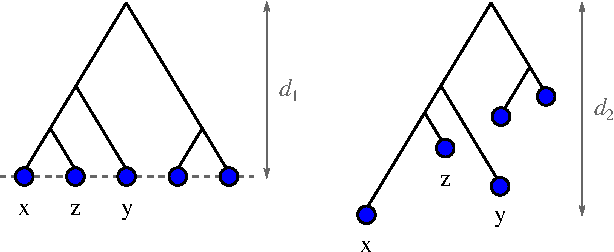
\includegraphics[width=0.65\columnwidth]{ultrametric_tree.pdf}
	\end{center}
	\caption[Ultrametric and non-ultrametric tree]{Ultrametric and non-ultrametric tree. The vertical components of the edges represent the distances. In the left tree, they induce an ultrametric on the set of its leaves, whereas they do not in the tree on the right side. This can, e.g., be seen by the violation of condition \textit{(iv*)} in Definition \ref{def:metric} for the leaves $x,y,z$: $d_2(x,y) > \max(d_2(x,z),d_2(z,y))$.}
	\label{fig:ultrametric_tree}
\end{figure}

In contrast, the distance function $d$ on the set of leaves $L(T)$ is not an ultrametric on the set of leaves in general. This is especially the case for evolutionary distances in the presence of asymmetric divergence as it will be discussed later. However, the distance function $d$ satisfies a weaker property by construction: A metric $d$ on set $X$ is \emph{additive} if a (not necessarily rooted) weighted tree $(T,\ell)$ exists such that $L(T)=X$ and $d=d_T$ where $d_T$ is the distance function of $(T,\ell)$ as defined by Equation~\ref{eq:distance_function}. A metric on a set $X$ can be tested for additivity with the four-point-condition: For any \emph{quartet}, i.e., a set of four nodes $x,y,u,v  \in X$, it must hold that out of the three distance sums
\begin{enumerate}[label=(\roman*), itemsep=0.2cm, topsep=0.2cm, parsep=0cm]
	\item $d(x,y)+d(u,v)$,
	\item $d(x,u)+d(y,v)$,
	\item $d(x,v)+d(y,u)$
\end{enumerate}
two sums are equal and not smaller than the third \citep[cf.][]{simoespereira1969,buneman1974}.

\begin{definition}[Quartet Relation {\citep[cf.][]{stadler2020}}]
	\label{def:quartet_relation}
	Consider an unrooted tree $\unrooted{T}$ with leaf set $L(\unrooted{T})$. For any four distinct leaves $x,y,u,v\in L(\unrooted{T})$ denote by $\unrooted{T}[x,y,u,v]$ the unrooted tree obtained by suppressing all vertices of degree $2$ in the union of the paths in $\unrooted{T}$ that connect $x,y,u,v$. The \emph{quartet relation} for $\unrooted{T}$ is
	\begin{enumerate}[label=(\roman*), itemsep=0.2cm, topsep=0.2cm, parsep=0cm]
		\item $\unrooted{T}[x,y,u,v]=(xy|uv)$,
		\item $\unrooted{T}[x,y,u,v]=(xu|yv)$ or
		\item $\unrooted{T}[x,y,u,v]=(xv|yu)$
	\end{enumerate}
	if there is an edge $e\in E(\unrooted{T})$ such that the respective pairs (that are separated by the vertical bar) are in different connected components of $\unrooted{T}$ after the removal of $e$. If there is no such edge write $\unrooted{T}[x,y,u,v]=\times$.
\end{definition}

The four-point-condition is directly related to this notion of quartets: For an additive metric $d$, the smallest of the three distance sums induced by four distinct points $x,y,u$ and $v$ determines their topology in a corresponding tree $\unrooted{T}$ that explains $d$. The reason for this is that the edge separating two pairs in $\unrooted{T}[x,y,u,v]$ only contributes to the two larger sums. The case in which all three sums are equal corresponds to the absence of such a separating edge in $\unrooted{T}$ (and hence also in $\unrooted{T}[x,y,u,v]$) and is referred to as \emph{star tree} or \emph{star topology}. The possible cases are visualized in Figure~\ref{fig:possible_quartets_unrooted}.

\vspace{5mm}
\begin{figure}[ht]
	\begin{center}     
		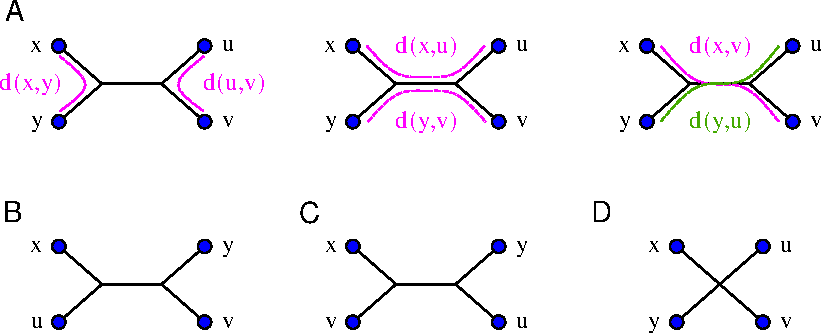
\includegraphics[width=0.9\columnwidth]{possible_quartets_unrooted.pdf}
	\end{center}
	\captionsetup{singlelinecheck=off}
	\caption[The four possible (unrooted) quartets]
	{The four possible (unrooted) quartets. For case (A), the six distances that form the three distance sums are indicated. In formal, the cases are:
		\begin{enumerate}[label=(\Alph*), itemsep=0.1cm, topsep=0.1cm, parsep=0cm]
			\item $\unrooted{T}[x,y,u,v]=(xy|uv)$ \newline $\iff d(x,y)+d(u,v) < d(x,u)+d(y,v) = d(x,v)+d(y,u)$
			\item $\unrooted{T}[x,y,u,v]=(xu|yv)$ \newline $\iff d(x,u)+d(y,v) < d(x,y)+d(u,v) = d(x,v)+d(y,u)$
			\item $\unrooted{T}[x,y,u,v]=(xv|yu)$ \newline $\iff d(x,v)+d(y,u) < d(x,y)+d(u,v) = d(x,u)+d(y,v)$
			\item $\unrooted{T}[x,y,u,v]=\times$ \newline $\iff d(x,y)+d(u,v) = d(x,u)+d(y,v) = d(x,v)+d(y,u)$
		\end{enumerate}
	}
	\label{fig:possible_quartets_unrooted}
\end{figure}

Given a rooted or unrooted tree $T$ and a unique numbering of the leaves $L(T)$, the distance function on the leaves can be represented by a symmetric square matrix which will be denoted by $\mathbf{D}$ in the following, where $\mathbf{D}(x,y)$ is the entry in the row and column corresponding to $x$ and $y$, respectively.



\subsection{Homology and Best Matches}
\label{sec:homology_and_bm}

As already outlined, the type of relationship between pairs of genes is of interest for the inference of gene functions. In particular, orthologous genes are considered to perform similar functions. Mathematically, both orthology and paralogy are binary relations on the set of (extant) genes in a gene tree $T$. They are defined w.r.t.\ the event type of the last common ancestor of two genes $x$ and $y$:

\begin{definition}[Orthology and Paralogy {\citep{fitch2000}}]
	\label{def:orthology}
	Let $(T,\mu,t)$ be an event-labeled, rooted gene tree with reconciliation map $\mu$.
	Two distinct leaves $x,y \in L(T)$ are \emph{orthologs w.r.t.\ $\mu$} if $t(\lca_T(x,y))=\SPEC$, and \emph{paralogs} if $t(\lca_T(x,y))=\DUPL$.
\end{definition}

Of course, the true reconciliation map and event-labeling are not known for real-life data. Therefore, methods exist that aim to explicitly reconstruct the gene tree and the reconciliation map, but also others that attempt to directly infer orthology based on gene similarity. In both cases, a well-founded mathematical investigation of the orthology and paralogy relation is helpful.

Firstly, Defintion~\ref{def:orthology} unambiguously defines two distinct members of a gene family as either orthologs or paralogs in the absence of horizontal gene transfer. Otherwise, there may be pairs of genes $x,y \in L(T)$ having a horizontal gene transfer as last common ancestor, and, thus, $t(\lca_T(x,y))=\HGT$.
Clearly, $x$ and $y$ are neither orthologs nor paralogs given the definition above. Therefore, \emph{xenology} was introduced as a third variant of homology. There are several definitions of xenologs. \citet{fitch2000} calls two genes xenologs if there is at least one HGT event on the unique path in $T$ connecting them. Thus, it is not necessary that their last common ancestor was an HGT event. As a consequence, two genes can be both xenologs and ortho-/paralogs. They are commonly termed as \emph{xeno-orthologs} and \emph{xeno-paralogs} in this case.
An alternative definition by \citet{hellmuth2016} avoids this ambiguity by calling two $x,y \in L(T)$ \emph{(lca-)xenologs} if and only if $t(\lca_T(x,y))=\HGT$. Analogously, \emph{(lca-)orthologs} and \emph{(lca-)paralogs} are defined. If not declared otherwise, all three terms will refer to this definition in the following.

Orthology and paralogy are irreflexive and symmetric binary relations, since for any $x\in L(T)$, it holds that $t(\lca_T(x,x))=t(x)=\LEAF$, and for any two genes $x,y\in L(T)$, $t(\lca_T(x,y)) = t(\lca_T(y,x))$. Hence, they can be represented by undirected graphs. However, they are not transitive, as the example in Figure \ref{fig:ortho_para_example} shows (consider, e.g., the three genes $a_1,b_1,c_1$ in the orthology graph $\Theta$).
\begin{definition}[Orthology Graph {\citep[Def. 5 mod.]{geiss2020c}}]
	Let $T$ be a gene tree with event labeling $t$. Let $\Theta$ be the undirected graph on $L(T)$ with $xy \in E(\Theta)$ if and only if $\lca_T(x,y)=\SPEC$. Then $\Theta$ is called an \emph{orthology graph} that is explained by the orthology relation of $(T,t)$.
\end{definition}
Similarly, the paralogy graph $\overline{\Theta}$ is defined. In the absence of HGT events, it is simply the complement of $\Theta$.

\vspace{5mm}
\begin{figure}[H]
	\begin{center}     
		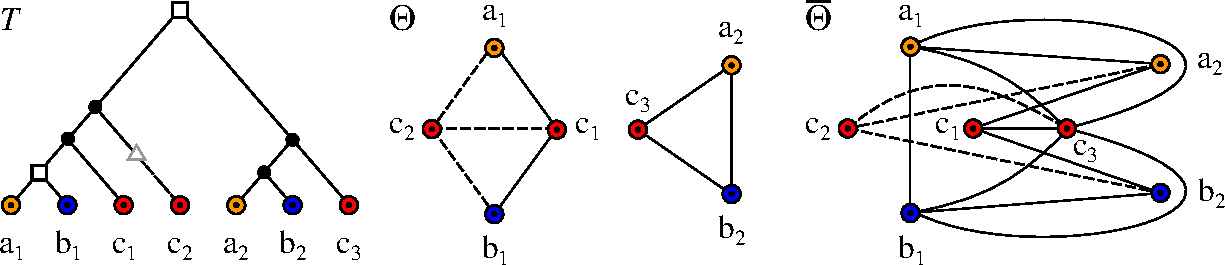
\includegraphics[width=\columnwidth]{ortho_para_example.pdf}
	\end{center}
	\caption[Example orthology graph $\Theta$ and paralogy graph $\overline{\Theta}$]{Corresponding orthology graph $\Theta$ and paralogy graph $\overline{\Theta}$ for the example gene tree in Figure \ref{fig:embedded_tree} restricted to the set of species $\{A,B,C\}$ (see tree $T$ on the left). Xeno-orthologous and \mbox{-paralogous} relations, respectively, are indicated by dashed lines.}
	\label{fig:ortho_para_example}
\end{figure}

Neither the orthology nor the paralogy relation can be observed directly. Therefore, heuristics have been developed that make use of the fact that orthologs are often the most closely related genes in two species. This approach has been used widely in phylogenetic reconstruction methods and requires some definition of the relationship between genes. To this end, different terms and variants have been introduced: Symmetric best matches \citep[e.g. used by][]{tatusov1997}, bidirectional best hits (BBH) \citep[e.g.][]{overbeek1999,lafond2018}, reciprocal best hits (RBH) \citep[e.g.][]{bork1998}, reciprocal best alignment heuristic (RBAH) \citep[e.g.][]{lechner2011} and some others.

We strictly distinguish between \emph{best hits} and \emph{best matches}:

\begin{definition}[(Reciprocal) Best hit]
	\label{def:best_hit}
	Consider a gene tree $T$ with leaf set $L(T)$, a surjective map $\sigma\colon L(T)\to L(S)$ (where $L(S)$ is the corresponding set of species) and a distance function $d:L(T)\times L(T)\to \mathbb{R}_0^+$.  Then $y\in L(T)$ is a \emph{best hit} of $x\in L(T)$ if and only if $d(x,y)\le d(x,y')$ holds for all leaves $y'$ from species $\sigma(y')=\sigma(y)$.\newline
	If $x$ is also a best hit of $y$, $x$ and $y$ are called \emph{reciprocal best hits}.
\end{definition}

Thus, \emph{best hits} are defined in the context of the smallest evolutionary distance. On the other hand, \emph{best matches} refer to the closest relatives of a gene w.r.t.\ the point in time when they were separated:

\begin{definition}[(Reciprocal) Best match {\citep{geiss2019a}}]
	\label{def:best_match}
	Consider a gene tree~$T$ with leaf set $L(T)$ and a surjective map $\sigma\colon L(T)\to L(S)$ (where $L(S)$ is the corresponding set of species).  Then $y\in L(T)$ is a \emph{best match} of $x\in L(T)$, in symbols $x\rightarrow y$, if and only if $\lca(x,y)\preceq \lca(x,y')$ holds for all leaves $y'$ from species $\sigma(y')=\sigma(y)$.\newline
	If $x$ is also a best match of $y$ in color $\sigma(x)$, i.e., $y\rightarrow x$, $x$ and $y$ are called \emph{reciprocal best matches}.
\end{definition}

A comprehensive mathematical theory on best matches was developed only recently by \citet{geiss2019a}. Therein, the authors point out that best hits and best matches are the same if the mutation rate of the gene family is constant, i.e., the \emph{Molecular Clock} holds.

The best match relation can be represented by a directed, vertex-colored graph on the set of leaves of a gene tree $T$ as follows:

\begin{definition}[cBMG and cRBMG {\citep{geiss2019a}}]
	\label{def:cBMG}
	Given a gene tree $T$ and a map $\sigma:L(T)\to L(S)$, the \emph{colored Best Match Graph (cBMG)} $\protect\G(T,\sigma)$ has vertex set $L(T)$ and arcs $(x,y)\in E(\protect\G)$ if $x\ne y$ and $x\rightarrow y$. Each vertex $x\in L(T)$ obtains the color $\sigma(x)$.  \newline The rooted tree $T$ \emph{explains} the vertex-colored graph $(\protect\G,\sigma)$ if $(\protect\G,\sigma)$ is isomorphic (in the usual sense, with preservation of colors) to the cBMG $\protect\G(T,\sigma)$.\newline
	The vertex-colored undirected graph $G(T,\sigma)$ that has vertex set $L(T)$ and edges $xy\in E(G)$ if $x\ne y$ and $x\rightarrow y$ as well as $y\rightarrow x$ is called the \emph{colored Reciprocal Best Match Graph (cRBMG).}
\end{definition}

\citet{geiss2019a} present two polynomial-time algorithms to decide whether a given digraph $(\G,\sigma)$ is a valid colored Best Match Graph and to determine the unique least resolved tree, i.e., the corresponding tree which explains $(\G,\sigma)$ and is minimal in the sense that no edge can be contracted such that the tree still explains $(\G,\sigma)$. The algorithm for computing the least resolved tree that will be relevant later in this contribution makes use of informative triples:

\begin{definition}[Informative triples {\citep[Def.~8]{geiss2019a}}]
	\label{def:inftriples}
	Let $(\protect\G,\sigma)$ be a two-colored digraph. We say that a triple $ab|c$ is \emph{informative} (for $(\protect\G,\sigma)$) if the three distinct vertices $a,b,c\in L$ induce a colored subgraph $\protect\G[a,b,c]$ isomorphic (in the usual sense, with preservation of colors) to the graph $X_1$, $X_2$, $X_3$ or $X_4$ shown in Figure~\ref{fig:triples}. The set of informative triples is denoted by $\mathscr{R}(\protect\G,\sigma)$.
\end{definition}

\vspace{5mm}
\begin{figure}[ht]
	\begin{center}     
		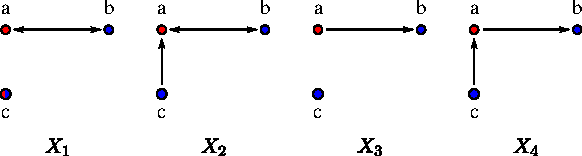
\includegraphics[width=0.7\columnwidth]{Triples.pdf}
	\end{center}
	\caption[Three-vertex induced subgraphs giving an informative triple]{Each of the three-vertex induced subgraphs $X_1$, $X_2$, $X_3$ and $X_4$ gives a triple $ab|c$. If vertex $c$ in the drawing has two colors, then the color $\sigma(c)$ does not matter \citep{geiss2019a}.}
	\label{fig:triples}
\end{figure}

This definition can easily be extended for n-colored graphs. \citet{geiss2019a} shows that the well-known polynomial-time algorithm \texttt{BUILD} \citep{aho1981} can be used to compute the least resolved tree directly from the full set of informative triples $\mathscr{R}(\protect\G,\sigma)$ of an n-colored Best Match Graph. Moreover, a colored digraph $(\G,\sigma)$ is a valid cBMG if and only if $(\G,\sigma) = \G(\textrm{Aho}(\mathscr{R}(\G,\sigma)),\sigma)$ where $\textrm{Aho}(\mathscr{R})$ denotes the tree $T$ that results from applying \texttt{BUILD} to a set of triples $\mathscr{R}$ \citep[][cf.~Theorems 6 and 9]{geiss2019a}. In other words, the Best Match Graph of the resulting tree has to be equal to the original digraph. Therefore, the explicit construction of a least resolved tree can be used to decide whether a given digraph is a cBMG.
%A more detailed description of Aho's \texttt{BUILD} algorithm and of the modification applied here will be given in the appropriate section (Section~\ref{sec:lrt_construction}).

\vspace{5mm}
In a subsequent publication, the properties of \emph{colored Reciprocal Best Match Graphs (cRBMG)} have been studied in detail \citep{geiss2020b}. Two genes $x$ and $y$ are reciprocal best matches if and only if both $x$ is a best match of $y$ and $y$ is a best match of $x$. As mentioned above, the cRBMG (possibly with some corrections based on the corresponding cBMG) is a good heuristic for the true orthology relation.
In fact, given a tree $T$ with reconciliation map $\mu$ and a corresponding event-labeling $t_\mu$, the orthology graph $\Theta(T,t_\mu)$ is a subgraph of the Reciprocal Best Match Graph $G(T,\sigma)$ \citep[Theorem~2]{geiss2020c} in the absence of horizontal gene transfer. Thus, the edges of $G$ cannot contain false positives w.r.t.\ the orthology relation.

Figure~\ref{fig:best_match_example} shows the cBMG $\G$, the cRBMG $G$ and the true orthology relation $\Theta$ that correspond to the previous example tree. The orthology graph is a subgraph of the cRBMG with exception of the xeno-orthologous relations. The simulations by \citet{geiss2020c} show that reciprocal best matches are a useful heuristic for orthology also if HGT occurs (at moderate rates).

\vspace{5mm}
\begin{figure}[ht]
	\begin{center}     
		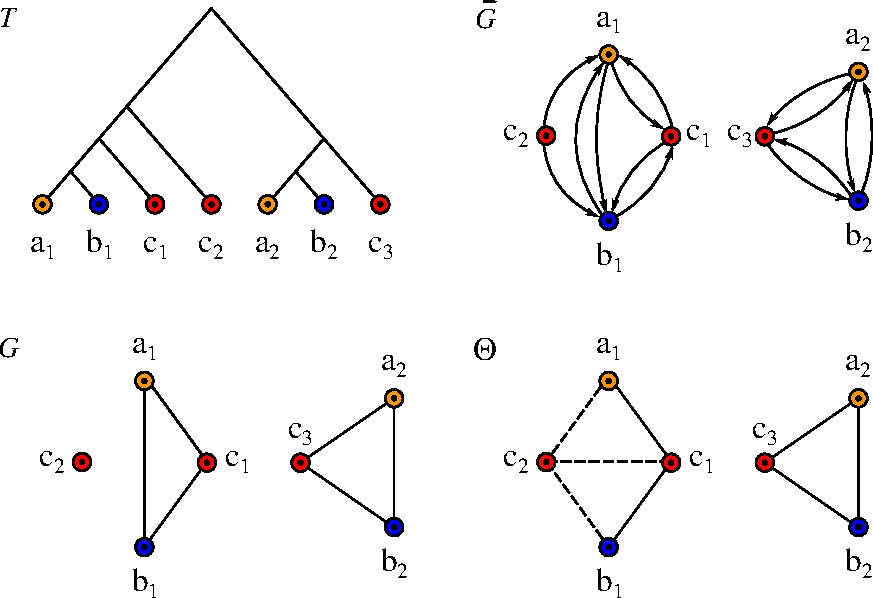
\includegraphics[width=0.65\columnwidth]{best_match_example.pdf}
	\end{center}
	\caption[Gene tree with corresponding cBMG and cRBMG]{Gene tree with corresponding colored Best Match Graph $(\G,\sigma)$ and Reciprocal Best Match Graph $(G,\sigma)$. The tree is a subtree of the gene tree in Figure~\ref{fig:embedded_tree} restricted to the set of species $\{A,B,C\}$. The true orthology graph $\Theta$ is again depicted for comparison.}
	\label{fig:best_match_example}
\end{figure}

However, especially in case of multiple losses, the true orthology relation is often hard to infer. The example includes the well-known problematic case of differential gene loss after a dupiclation event followed by speciation. The last common ancestor of genes $a_1$ and $b_1$ is a duplication (see Figure \ref{fig:embedded_tree}). The two loss events cause a false-positive edge when considering $G$ as the estimated orthology relation.
%It will be discussed later how the Best Match Graph can help resolve this issue in some cases (see Section~\ref{sec:role_best_matches}).

\section{Simulation of Gene Family Histories}
\label{sec:simulation}

In the first two sections of this chapter, the methods for the simulation of dated species and gene trees are described. They are based on the methods used by \citet{hernandez-rosales2014} and \citet{lopezsanchez2019}. They generate the gene trees by constructing Poisson vectors of events for the edges of the species tree $S$, whereas a variant of the Gillespie algorithm \citep{gillespie1976} is used here.

In the rest of the chapter, the simulation of evolution rate imbalances and measurement noise is discussed. The former is a result of the divergent fates of genes after their separation by speciation, duplication or horizontal gene transfer, and is therefore commonly observed in biological data. For the distances of the leaves of $T$, this destroys the property of ultrametricity. An overview of the simulation framework is supplied in Figure~\ref{fig:simulation_framework}.

\vspace{5mm}
\begin{figure}[ht]
	\begin{center}     
		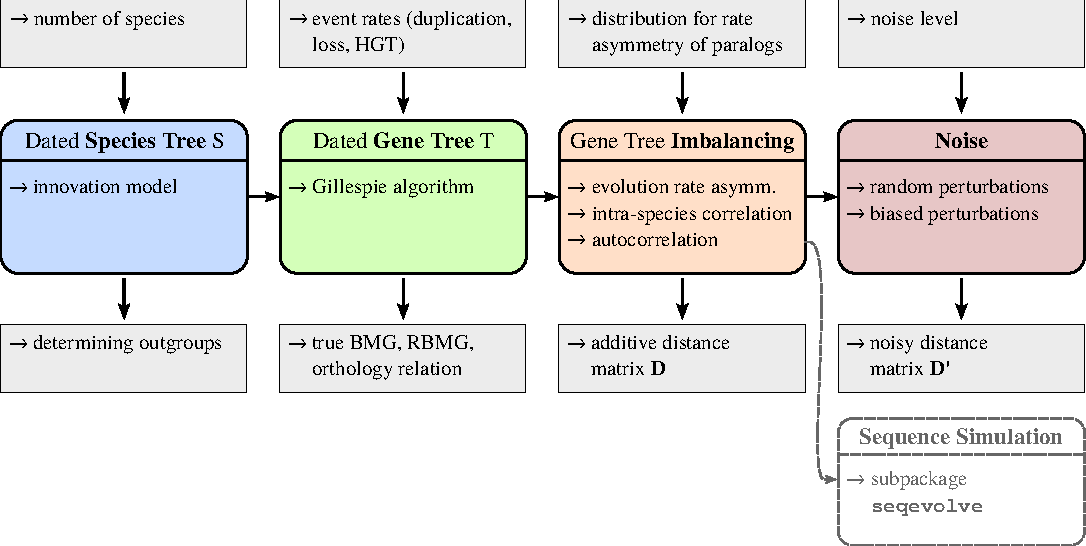
\includegraphics[width=\columnwidth]{simulation_framework.pdf}
	\end{center}
	\caption[Overview of the framework for the simulation of realistic evolutionary distance data]{Overview of the framework for the simulation of realistic evolutionary distance data. The four main modules are indicated by the colored boxes, the most important input as well as some additional output data above and below, respectively.}
	\label{fig:simulation_framework}
\end{figure}

Moreover, in Fig.~\ref{fig:simulated_trees}, an example for a simulated scenario is shown including a species tree, an imbalanced gene tree and the corresponding observable gene tree, i.e., the gene tree after removing all branches that lead to loss events only and then suppressing all inner vertices that have only one child.

\vspace{5mm}
\begin{figure}[ht]
	\begin{center}     
		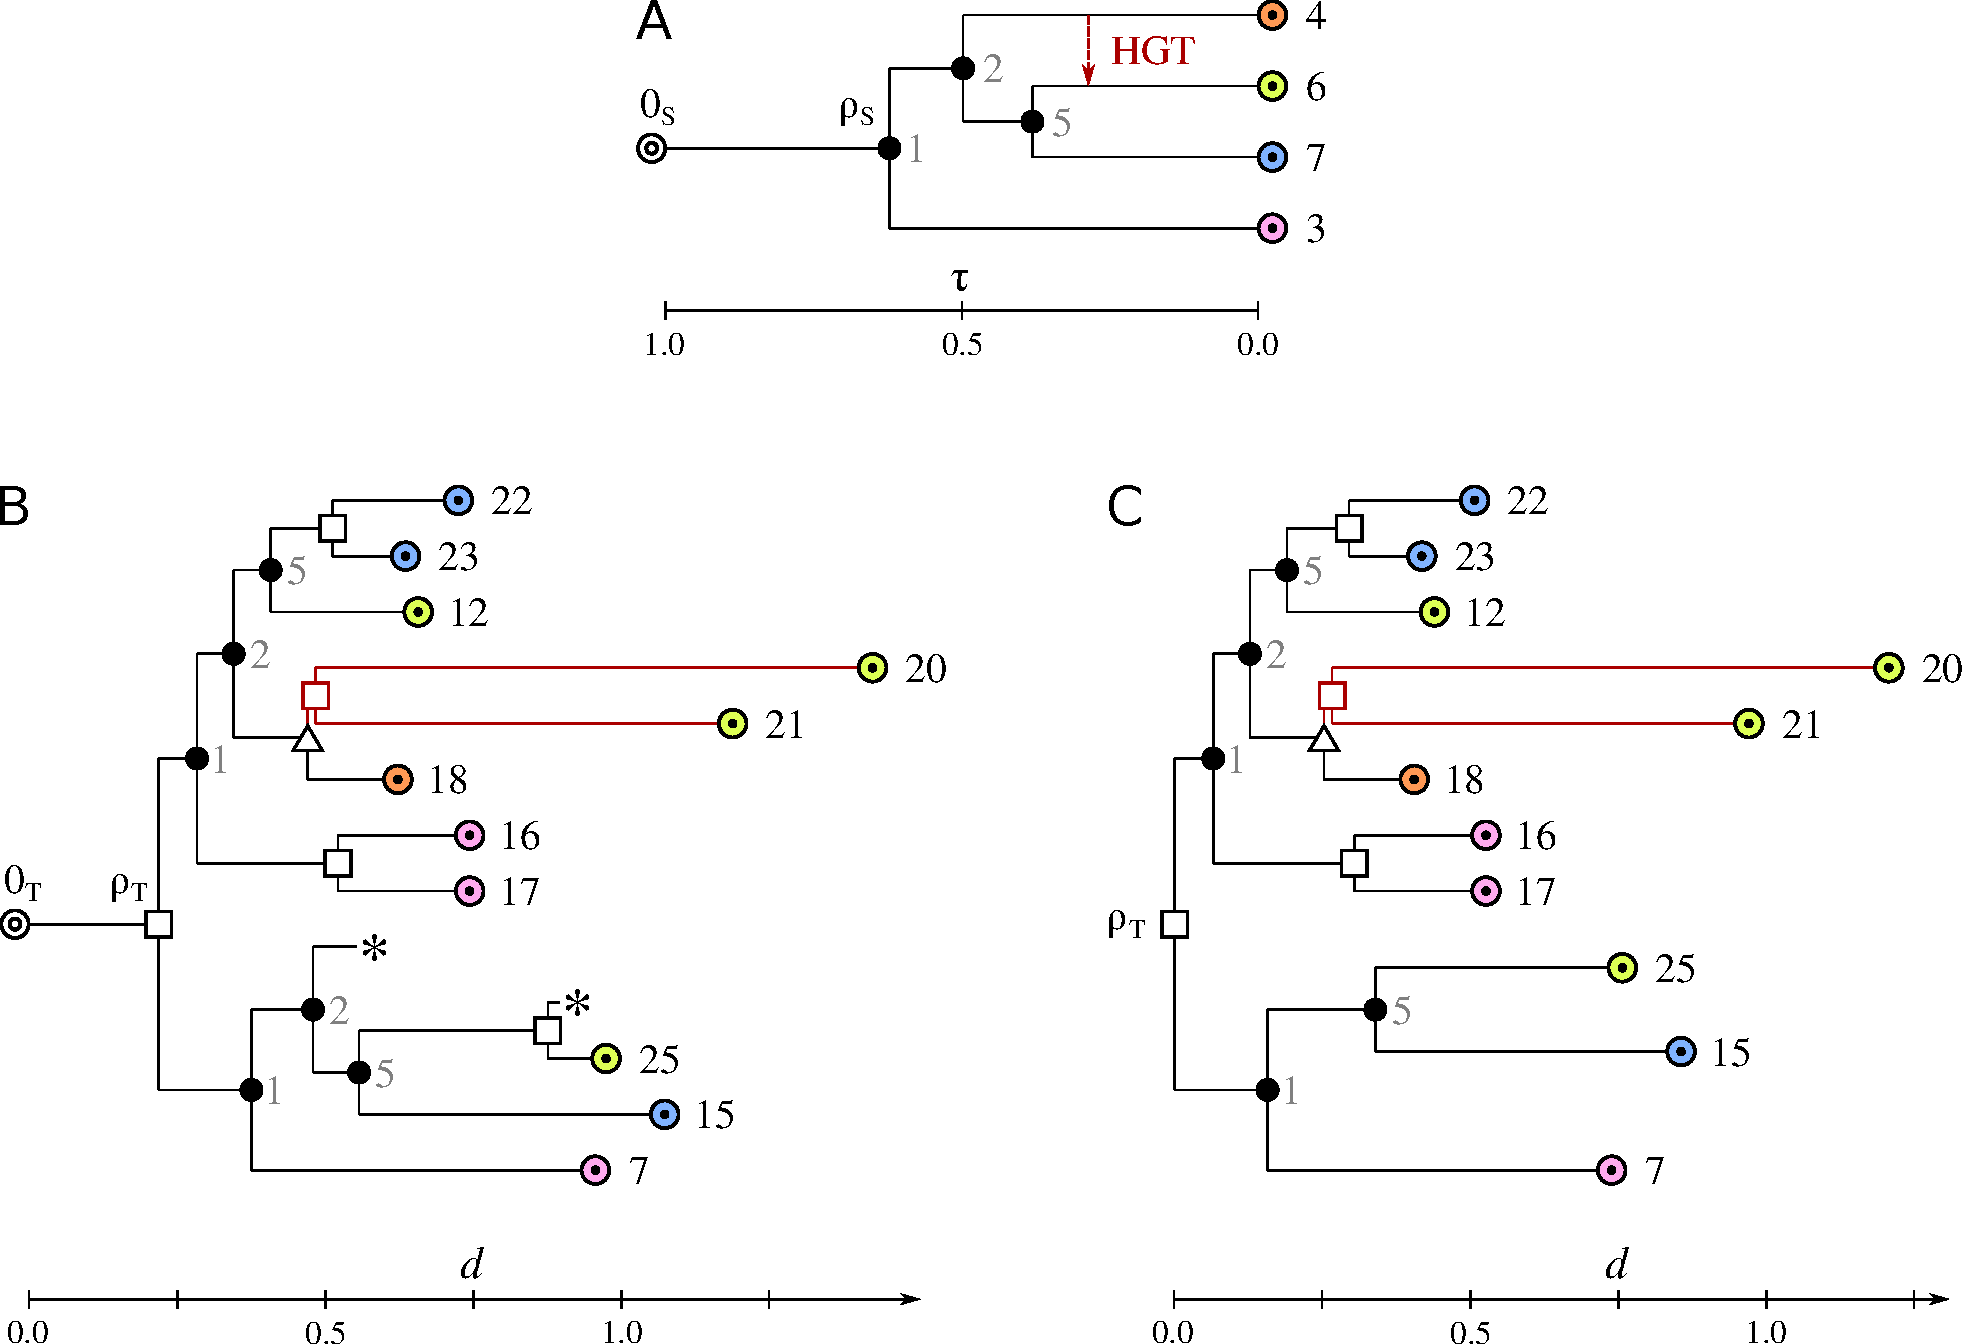
\includegraphics[width=\columnwidth]{simulated_trees.pdf}
	\end{center}
	\caption[Example simulated species tree and imbalanced gene tree]{Example simulated species tree and imbalanced gene tree. (A) Planted species tree on four (extant) species. The dating function is represented by the scale below. (B) Extended gene tree, i.e., the complete history of the simulated gene family including speciations ($\SPEC$), duplications ($\DUPL$), losses ($*$)  and an HGT event ($\HGT$; transferred branch in red). The numbers at the speciation events correspond to the numbering in (A), the numbers at the leaves are their unique IDs. The leaf coloring indicates the corresponding species. The scale represents the evolutionary distance from the root $0_T$. The lengths of the horizontal lines are all to scale. (C) Observable gene tree.}
	\label{fig:simulated_trees}
\end{figure}

\subsection{Simulation of Species Trees}
\label{sec:species_tree}

The \emph{innovation model} described by \citet{keller-schmidt2012} produces tree topologies that are comparable with those of real phylogenetic trees considering properties like average leaf depth and tree imbalance. It assumes that that evolutionary branching is driven by innovations, i.e., the generation of novel features or the loss of such features.

In order to produce realistic gene family histories, the species tree $S$ has to meet some additional requirements. Firstly, it is possible that events, such as gene duplications or losses, predate the first speciation event in biological gene trees. Therefore, an additional node $0_S$ is added to $S$ and connected to the first speciation event $\rho_S$. Hence, in the following generation of gene trees $T$ along the planted species tree $S$, events can already occur within the edge $0_S\rho_S$.

Secondly, a dating function $\tau: V(S) \rightarrow [0,1]$ has to be constructed to introduce a realistic variance for the time intervals between speciation events and to determine the set of available edges for a given time~$\tau$ (especially in the wake of HGT). For the construction of the dating function $\tau$, the tree is traversed in pre-order and the following rules are applied:
For each $v \in V(S)$, set $\tau(v)=1$ if $v=0_S$, $\tau(v)=0$ if $v$ is a leaf. Otherwise, pick a random leaf $l \in L(S(v))$ and determine the length of the path $P$ (i.e., the number of edges $|P|$) from $v$ to $l$. Next, a random number $r$ is drawn from a uniform distribution on the interval $[0,2]$. It is used to introduce more variability into the lengths of the edges by setting $\tau(v) = \tau(u) \cdot r / (|P|+1)$. In this equation, $u$ is the parent of $v$. The pre-order traversal ensures that $\tau(u)$ is already set for any $v \in V(S)\setminus\{0_T\}$. The procedure is summarized in Algorithm \ref{alg:ultrametric}.

\begin{algorithm}
	\caption{Construction of the dating function for $S$}
	\label{alg:ultrametric}
	\SetAlgoLined
	\DontPrintSemicolon
	\KwData{(Optionally planted) species tree $S$}
	\KwResult{Dating function $\tau$.}
	\ForEach{$v \in V(S)$ in pre-order}{
		\uIf{$\parent(v)=\emptyset$ (root)}{
			Set $\tau(v)=1$.\;
		}
		\uElseIf{$|\child(v)|=0$ (leaf)}{
			Set $\tau(v)=0$.\;
		}
		\Else{
			Draw a random leaf $l \in L(S(v))$.\;
			Determine the length of the path $P$ between $v$ and $l$.\;
			Draw $r \in [0,2]$ uniformly.\;
			Set $\tau(v) = \tau(\parent(v)) \cdot r / (|P|+1)$.\;
		}
	}
	
\end{algorithm}

Note that the algorithm also works for unplanted trees which are normalized such that $\tau(\rho_S)=1$. The length of each edge $uv \in E(S)$ in the resulting dated species tree (in the sense of divergence time) is given by $\tau(u)-\tau(v)$. Furthermore, $(S, \tau)$ induces an ultrametric on the set of leaves $L(S)$ as described in Section~\ref{sec:metrics}.


\subsection{Simulation of Gene Trees}
\label{sec:gene_tree_sim}

\subsubsection{The Gillespie Algorithm}

The history of a gene family is embedded into the phylogeny of the corresponding species tree. Mathematically, this relationship is formalized in the reconciliation map $\mu:V(T)\to V(S)\cup E(S)$ which was described in Section \ref{sec:phylogenetic_trees}.
Whenever a speciation event, resulting in two separated branches in $S$, occurs, the evolutionary histories of all genes in the ancestral species are also separated. Additionally, duplication, horizontal gene transfer, and loss events occur with certain rates during the evolution of the species, which also lead to branching in the gene tree $T$ or termination of branches in the latter case.

Whilst the speciation events are fixed by $S$, the Gillespie algorithm is a suitable choice for the exact stochastic simulation of events occurring with rates that may depend on the current state of the system. First introduced by Daniel Gillespie in 1976, the algorithm is best known for the simulation of chemical reaction kinetics in systems with relatively small numbers of molecules. Traditional methods that assume the number of reactants to be continuous fail in this situation \citep{gillespie1977}.

In the original description \citep{gillespie1976}, the overall simulation algorithm consists of the following (here slightly simplified) steps:
\begin{itemize}
	\item \textit{Step 1: Initialization}\\
	Initialize the time to $\tau=0$ and the molecule numbers $X_1, X_2, ..., X_N$ for a set of $N$ chemical species. Furthermore, specify the rates $r_1, r_2, ..., r_M$ for a set of $M$ possible reactions ($\xi_1, \xi_2, ..., \xi_M$) between these reactants. The rates are usually functions of the $X_1, X_2, ..., X_N$. Determine a stopping time $\tau_{\textrm{stop}}$.
	\item \textit{Step 2: Monte-Carlo-Step}\\
	Generate a random pair $(\Delta\tau,\mu)$ according to the joint probability function $P(\Delta\tau,\mu)$ where $\Delta\tau$ is the waiting time until the next event and $1\le\mu\le M$ an integer deciding which of the $M$ reactions will occur next.
	\item \textit{Step 3: Update}\\
	Advance $\tau$ by $\Delta\tau$. Update the values of the chemical species $X_1, X_2, ..., X_N$ according to one occurrence of reaction $\xi_\mu$ as well as the reaction rates $r_1, r_2, ...,\allowbreak r_M$.
	\item \textit{Step 4: End of iteration}\\
	Terminate the simulation if $\tau>\tau_{\textrm{stop}}$ or no more reactions can occur, i.e., all rates $r_1, r_2, ..., r_M$ are zero. Otherwise, return to Step 2.
\end{itemize}

For the correct generation of $\Delta\tau$ and $\mu$ in the Monte-Carlo-Step, Gillespie proposes two methods which he proofs to be equivalent: the `Direct' and the `First reaction' method.
In the `Direct' method, a total rate $R$ is computed for each iteration step as
\begin{equation}\label{eq:total_rate_R}
R = \sum_{\mu=1}^{M}r_\mu.
\end{equation}
Next, two random numbers $x_1$ and $x_2$ are drawn from a uniform distribution over the interval $(0,1]$ and $\Delta\tau$ is set to
\begin{equation}
\Delta\tau = (1/R) \ln(1/x_1).
\end{equation}
Finally, the reaction $\xi_\mu$ is selected such that
\begin{equation}\label{eq:reaction_selection}
\sum_{\nu=1}^{\mu-1}r_\nu < x_2 R \le \sum_{\nu=1}^{\mu}r_\nu.
\end{equation}
For the `First reaction' method, individual waiting times $\Delta\tau_\nu$ are drawn for each of the $M$ reactions again using random numbers $x_\nu$ and setting
\begin{equation}
\Delta\tau_\nu = (1/r_\nu) \ln(1/x_\nu) \qquad (\nu = 1,2,...,M).
\end{equation}
Thus, a random number $x_\nu$ has to be drawn for every reaction. The next reaction $\xi_\mu$ with the corresponding waiting time $\Delta\tau_\mu$, that is actually carried out, is then chosen such that $\Delta\tau_\mu$ is smallest among the $\Delta\tau_1,\Delta\tau_2,...,\Delta\tau_M$.

\citet{gillespie1976} shows that both approaches are equivalent and correct implementations of the Monte-Carlo-Step w.r.t.\ the probability function $P(\Delta\tau,\mu)$. In both cases, the waiting time $\Delta\tau$ follows an exponential distribution with rate $R$ as given by Equation~\ref{eq:total_rate_R}.
However, for the simulation of events along a species tree, some additional considerations have to be made which are described in the next section.

The Gillespie algorithm has previously been used for the simulation of gene family histories, e.g., in the Artificial Life Framework \citep[\texttt{ALF},][]{dalquen2012}, in which the set of possible events comprises duplications and losses, but also indels and substitutions in DNA sequences. This way, the evolution on the genome and sequence level is simulated in parallel.

\subsubsection{Implementation}

The Gillespie algorithm was originally designed for non-branching processes. For example, in the simulation of chemical reactions, the assumption is made that all molecules are contained in a defined volume and are therefore not restricted from interacting with one another \citep{gillespie1977}.
In gene family histories, on the other hand, genes are separated by branching events such as speciations and duplications. The simulation procedure must therefore also enable branching in some way. It appears, in particular, that the order in which single branches are handled is relevant whenever dependencies exist, i.e., as well as chemical reactions in the original version, events can result in changes of rates.

Especially, the extinction of a whole gene family in a species should be avoided. It is thus necessary to keep track of the current number of genes in all species and set the loss rate $l_g=0$ whenever gene $g$ is the only copy in its species. Likewise, duplications and horizontal gene transfers (HGTs) can reset $l_g$, e.g., to some initially specified default value in the simplest case.

In this section, a variant of the Gillespie algorithm is described that is able to correctly handle the above-described cases. Moreover, it can be interpreted as a more stringent application of the `Direct' method as compared to an alternative implementation in the next section. It is therefore also referred to as the \emph{Direct method} here.

As a first modification to the original algorithm by \citet{gillespie1976}, the set of possible reactions is not fixed, but it is updated after every event instead. The reason for this is that all combinations of extant genes at a given time $\tau$ and event types are considered as the reactions, i.e., they are given by the Cartesian product $G(\tau) \times Q$ where $G(\tau)$ is the set of \emph{active} genes, i.e., every $g\in G(\tau)$ is an extant gene at time $\tau$, and $q\in Q\coloneqq\{D,L,H\}$ is one of the three events duplication, loss and HGT.
Hence, the reactions $\xi \coloneqq (g,q)$ correspond to the possible simulation events excluding speciations. Furthermore, they are associated with a rate $r_{\xi}(\tau)$ that depends on the time $\tau$. In particular, for the default settings, $r_{\xi}(\tau)$ will either be $0$ or $l$ if $q=L$, where $l$ is a user-defined default loss rate. If $q\in\{D,H\}$ on the other hand, the rate will be equal to some fixed duplication rate $d$ or HGT rate $h$, respectively. For each time point $\tau$, the total event rate $R(\tau)$ is thus given by
\begin{equation}
R(\tau) = \sum_{\xi \,\in\, G(\tau) \times Q} r_{\xi}(\tau).
\end{equation}

The simulation is initialized by setting $\tau=1$ and $\tau_{\textrm{stop}}=0$. Recall that $\tau(0_S)=1$ and that the time decreases as the simulation progresses towards the leaves. All speciation events are kept in a priority queue $\mathcal{P}$ in temporal order. This is possible because they are known \textit{a priori} from the dated species tree $S$. A single gene $g_{0}$ is associated with the planted edge $0_S\rho_S$ in $S$ and added to the set of active genes.
The total event rate is computed as $R(1) = d+h$, since losses are not allowed for a single gene. Note that, effectively, HGT events also cannot yet be carried out, since there is only a single species (see below).

In each iteration, first, a random number $\Delta\tau$ is drawn from an exponential distribution with rate parameter $R(\tau)$ representing the waiting time until the next duplication, loss or HGT event.
Next, it is checked whether the interval $[\tau, \tau - \Delta\tau]$ contains the time point $\tau_s$ of the first element in the queue $\mathcal{P}$ containing the speciation events. If this is the case, the speciation is given priority and removed from the queue. The time $\tau$ is hence updated to $\tau_s$ and gene copies $g_1,...,g_n$ of \emph{each} parental gene $g$ are placed into the respective edges $e_1,...,e_n$ below the speciation event in $S$ (where $n$ is the number of children of the corresponding vertex in $S$). The copies $g_1,...,g_n$ are associated with the event rates of the respective parental gene and added to the set of active genes, whereas the parental genes are removed from it.

Since the number of active genes has increased and thus also $R(\tau)$, a new waiting time $\Delta\tau'$ until the next event has to be drawn in the next iteration.
This is the correct way of handling the situation, since the stochastic process of Gillespie's algorithm is essentially a first order Markov process \citep{bustin2006}, i.e., all probabilities solely depend on the current state of the system and are independent from the past.
In particular, the distribution of waiting times from a time point $\tau_0$ until the next event conditioned on the fact that no event occurred between $\tau_0$ and $\tau_s$, where $\tau_0$ designates the time before it was updated to $\tau_s$, can be expressed as follows: Consider the complementary cumulative distribution function and let $\sigma \coloneqq \tau_0-\tau_s$: 
\begin{equation}
\begin{aligned}
\mathbb{P}(T \ge \sigma+\Delta\tau' |  T \ge \sigma) & =
\mathbb{P}(T \ge \sigma+\Delta\tau' \wedge T \ge \sigma)/\mathbb{P}(T\ge \sigma) \\
& = \mathbb{P}(T \ge \sigma + \Delta\tau')/\mathbb{P}(T \ge \sigma).
\end{aligned}
\end{equation}
The waiting time distributions are exponential with rate $R_1 \coloneqq R(\tau_0)$ before $\tau_s$ and rate $R_2 \coloneqq R(\tau_s)$ following the speciation event. Moreover, the event (in the sense of the sample space) that nothing happened in the time interval $[\tau_s, \tau_s-\Delta\tau']$ is independent from the event that nothing happened in $[\tau_0, \tau_0-\sigma]$. 
Hence, one obtains
\begin{equation}
\mathbb{P}(T \ge \sigma+\Delta\tau' |  T \ge \sigma) = \frac{\exp{\left[-R_1 \sigma \right]}\exp{\left[-R_2 \Delta\tau'\right]}}{ \exp{\left[-R_1 \sigma\right]}} =
\exp{\left[-R_2\Delta\tau'\right]}  .
\end{equation}
The distribution of the waiting time after the speciation event is thus equal to an exponential distribution with rate parameter $R_2$. It is the same that will be used in the following iteration.

In case there is no speciation event interfering with the time interval $[\tau, \tau - \Delta\tau]$, the time is updated according to $\tau \leftarrow \tau - \Delta\tau$. If $\tau < \tau_{\textrm{stop}}=0$, the iteration is ended. Otherwise, a second random number $x$ is drawn from a uniform distribution on the unit interval and is then used to select the upcoming reaction, i.e., the active gene and event type.
The probability for each reaction is equal to $r_{\xi}(\tau)/R(\tau)$ and the implementation follows the suggestion in the original algorithm (see  Equation~\ref{eq:reaction_selection}). The iteration proceeds depending on the selected gene $g$ and event type $q$:
\begin{itemize}
	%\setlength\itemsep{0cm}
	\item \textit{Duplication ($q=D$)\\}
	A gene duplication is modeled by placing a new copy $g'$ into the same branch of $S$, i.e., the edge $e \in E(S)$ that embeds $g$, and adding $g'$ to the set of active genes.
	\item \textit{Loss ($q=L$)\\}
	A gene loss is modeled by removing $g$ from the set of active genes.
	\item \textit{HGT ($q=H$)\\}
	A horizontal gene transfer is modeled by choosing a target edge $e'$ uniformly from all coexisting branches in $S$ at time $\tau - \Delta\tau$ (excluding the branch in which $g$ resides). If such an edge does not exist, nothing is done. Otherwise, a copy $g'$ is placed into edge $e'$ and added to the set of active genes.
\end{itemize}
In general, the rates $\xi_{(g,q)}(\tau - \Delta\tau)$ and $\xi_{(g',q)}(\tau - \Delta\tau)$ are set to $\xi_{(g,q)}(\tau)$. However, in the wake of restricting the extinction of the gene family, some special cases have to be considered:
\begin{itemize}
	\item \textit{Setting the loss rate to zero\newline}
	If a loss event is performed leaving gene $g^*$ as the last survivor in its species, then set $\xi_{(g^*,L)}(\tau - \Delta\tau) = 0$.
	\item \textit{Resetting the loss rate\newline}
	(i) If a duplication is performed, where $g$ was the last survivor in its species, then reset $\xi_{(g,L)}(\tau - \Delta\tau) = \xi_{(g',L)}(\tau - \Delta\tau) = l$ where $l$ is the user-defined default loss rate.\newline
	(ii) If a HGT is performed, where $g$ was the last survivor in its species, then reset $\xi_{(g,L)}(\tau - \Delta\tau) = l$. In any case, set $\xi_{(g',L)}(\tau - \Delta\tau) = l$ for HGTs.
\end{itemize}
The simulation is finished as soon as $\tau < \tau_{\textrm{stop}}=0$. The construction of the dated gene tree $T$ is done in parallel, i.e., vertices for every type of event are added, associated with the corresponding time stamp and connected to the correct parent node. After the last iteration, a leaf $l_g$ with time stamp $\tau(l_g)=0$ is added to $T$ for all active genes $g\in G(0)$. Also, the reconciliation map between $T$ and $S$ is saved as a by-product. The complete simulation is summarized in Algorithm~\ref{alg:gillespie_direct}.

\vspace{5mm}
{\normalsize
	\begin{algorithm}[H]
		\caption{Direct Gillespie algorithm for the simulation of $T$}
		\label{alg:gillespie_direct}
		\SetAlgoLined
		\DontPrintSemicolon
		\Input Planted species tree $S$, default event rates $d$, $l$ and $h$ \;
		\Output (Extended) Gene tree $T$ and reconciliation map $\mu$ \;
		Initialize gene tree $T$ with root $0_T$ and reconciliation map $\mu$.\;
		Set $\tau=1$ and $\tau_{\textrm{stop}}=0$.\;
		Initialize a priority queue $P$ with the speciation events in temporal order.\;
		Initialize set of active genes $G$ with a single copy in the planted root of $S$, and the total rate $R=d+h$.\;
		\While{$\tau > \tau_{\textrm{stop}}$}{
			Draw $\Delta\tau$ from an exponential distribution with rate $R(\tau)$.\;
			\uIf{$\tau - \Delta\tau<\tau_s$ where $\tau_s$ is the time of the next speciation event}{
				Set $\tau=\tau_s$.\;
				Pop the next speciation event $s$ at the front of $P$.\;
				Add copies $g_1,...,g_n$ for \emph{all} parental genes $g$ into the corresponding edges below $s$ and into $G$.\;
				Remove the parental genes $g$ from $G$.\;
				Add a speciation vertex $v$ for every parental gene $g$ and the edge $uv$ from its ancestor $u$ to $T$.\;
			}
			\uElseIf{$\tau - \Delta\tau < \tau_{\textrm{stop}}$}{
				Set $\tau \leftarrow \tau - \Delta\tau$.\;
				\Continue\;
			}
			\Else{
				Set $\tau \leftarrow \tau - \Delta\tau$.
				Draw a random number $r$ from a uniform distribution on $[0,1]$.\;
				Select reaction $\xi=(g,q)$ using $r$.\;
				\uIf{$q=D$}{
					Add a copy $g'$ of $g$ into the same branch of $S$ and to $G$.\;
				}
				\uElseIf{$q=L$}{
					Remove $g$ from $G$.\;
				}
				\uElseIf{$q=H$}{
					\uIf{another branch exists in $S$}{
						Select a coexisting branch in $S$ and add a copy $g'$ of $g$ into it and into $G$.\;
					}
					\Else{
						\Continue\;
					}
				}
				Add a vertex $v$ for the event to $T$ and the edge $uv$ from its ancestor $u$.\;
			}
			Update all rates $r_\xi(\tau)$ and $R(\tau)$.\;
			Update the reconciliation map $\mu$.\;
		}
		Add a leaf $l_g$ for every gene $g\in G$ to $T$, and the edge $ul_g$ from its ancestor $u$.\;
\end{algorithm}}

\newpage


\subsection{Divergence Asymmetries}
\label{sec:divergence_asym}

\subsubsection{Motivation}

In Section~\ref{sec:gene_tree_sim}, the simulation of dated gene trees has been described. As already introduced in the preliminaries section, the normalized dating function $\tau: V(T) \rightarrow [0,1]$ induces an ultrametric divergence time $d_\tau$ between the non-loss leaves of the gene tree which is given by
\begin{equation}
d_\tau(x,y) = 2 \tau(\lca_T(x,y)).
\end{equation}
For biological data, divergence times cannot be observed directly in most cases. Similarities or dissimilarities of nucleic or amino acid sequences are therefore used to approximate the relatedness of genomic regions.
The \emph{Molecular Clock Hypothesis}, which was first described in the early 1960s, states that genes evolve with a constant mutation rate \citep{zuckerkandl1962}. In this case, for a constant substitution rate $r$ the genetic distance $d$ of two genes $x$ and $y$ would be given by $d(x,y) = 2 r \tau(\lca_T(x,y))$. It can easily be seen that such distances are still ultrametric.
The theory has been shown to be a remarkably good approximation for many gene families and it is a key assumption for numerous bioinformatics algorithms and tools \citep[e.g.][]{bromham2003,kumar2005}.

However, the \emph{Molecular Clock Hypothesis} fails in the presence of the well-known phenomenon of asymmetric divergence after gene duplication.
The first attempt to explain unequal mutation rates of two paralogs after their separation was \emph{Ohno's neofunctionalization} model \citep{ohno1970}. He suggested that, after the duplication, one copy will maintain its original function, while the other becomes relieved from negative selective pressure and therefore accumulates mutations. In many cases, the redundant copy would get lost again or pseudogenized, but in other cases, the mutations might lead to the acquisition of new functions that can be completely different from the original one. An example supporting this theory is the evolution of an antifreeze protein from a duplicated sialic acid synthase gene in an Antarctic zoarcid fish enabling it to survive in colder environments than related species \citep{deng_evolution_2010}.

Another very prominent model for divergence after duplication is the \emph{Du\-pli\-ca\-ti\-on-de\-ge\-ne\-ra\-ti\-on-com\-ple\-men\-t\-ati\-on (DDC)} model by \citet{force1999}. There, it is assumed that both copies accumulate mutations in the first phase after duplication as a result of reduced selective pressure (`degeneration phase'). As a consequence, one copy alone can no longer fulfill its original function sufficiently. Rather, they divide the function either on the level of regulation by differential gene expression or on the level of gene products, i.e., the proteins or functional RNAs differ in their functionality. Either way, both copies are needed (`complementation') and must be maintained by selection. The model makes different predictions for the evolution rates after duplication. In the degeneration phase, both copies should show an increased, but approximately equal mutation rate. In the complementation phase, they are again exposed to a negative selective pressure leading to either equal or asymmetric divergence depending on the functions and the specific case.

A closely related theory is the \emph{specialization} model \citep{hughes1994,desmarais2008}. It proposes that genes can suffer from a so-called adaptive conflict, i.e., the gene is fulfilling two or more functions and is therefore constrained from optimizing either one of them since this would lead to a degeneration of the others. Hence, a duplication might allow the \emph{escape from adaptive conflict (EAC)} and specialization for single functions. As before, the extent of mutation rate asymmetries is case-dependent.

So far, all models predict that at least one of the duplicates acquires new functions. However, there are also known cases in which an increased gene dosage after duplication confers an immediate selective advantage to a species \citep{kondrashov2002,conant2007}. The original function is therefore maintained by both copies and the (possibly relaxed) selective pressure affects them both equally.

Numerous other models and extensions to the above-described ones have been proposed, a number of which have been reviewed e.g.\ by \citet{innan2010}, where the summary in Table~\ref{table:dupl_models} is taken from.

\begin{table}[h]
	\centering
	\setlength{\tabcolsep}{6pt}
	\renewcommand{\arraystretch}{1.5}
	\renewcommand\tabularxcolumn[1]{m{#1}}
	\begin{tabularx}{\textwidth}{|m{2.5cm}|m{2.2cm}|m{2.2cm}|m{2.2cm}|Y|Y|}
		\hline
		& \multicolumn{3}{c|}{\textbf{Function}} & \multicolumn{2}{c|}{\textbf{Evolution rate}}\\
		\cline{2-6}
		\centering \textbf{Model} & \centering Original copy & \centering New copy &  \centering Fate-determining mutation & Original copy & New copy \\
		\hline
		Neofunc-tionalization & Kept & Novel & Gain-of-function
		mutations & $\alpha$ & $\beta$ \\ 
		DDC & Subfunc-tionalized & Subfunc-tionalized & Loss-of-function
		mutations & $\beta$ & $\beta'$ \\
		Specialization (EAC) & Subfunc-tionalized & Subfunc-tionalized & Gain-of-function
		mutations & $\beta$ & $\beta'$ \\
		Positive dosage & Kept & Same as\newline original & Not\newline applicable & $\alpha'$ & $\alpha'$\\
		\hline
	\end{tabularx}
	\caption{Summary of the models of gene-duplication evolution (excerpt and modified from \citet{innan2010}). The rate $\alpha$ represents the pattern in the pre-duplication phase, where $\alpha'$ indicates a possibly relaxed selective pressure. Accelerated non-synonymous mutation rates (i.e., mutations leading to amino acid substitutions) are indicated by $\beta$ and $\beta'$.}
	\label{table:dupl_models}
\end{table}

It has to be remarked, that all of these models do not exclude one another, i.e., gene duplication scenarios in biological systems could either be combinations of several models, as e.g.\ found by \citet{teufel2016}, or they could simply coexist. In the latter case, it is likely that all (or at least most) theories have their counterparts in biology.

Anyways, asymmetric divergence rates have been observed in a large number of clades ranging from simple eukaryotes like yeast \citep{kellis2004,byrne2007,scannell2007}, invertebrates like \textit{Drosophila} \citep{assis2013} to chordates \citep{brunet2006,hellsten2007,assis2015,nembaware2002}. In order to produce realistic gene history scenarios, it is therefore necessary to take into account unequal divergence after gene duplication.


\subsubsection{Divergence After Gene Duplication}

To estimate the divergence asymmetry between pairs of paralogs, the sequence divergence to a member of the gene family in a closely related species has to be determined. Commonly used measures of sequence divergence are the rate of synonymous nucleic acid exchanges $K_S$ and the rate of non-synonymous (or amino acid) exchanges $K_A$ \citep{kellis2004,byrne2007,assis2015}.

Whilst synonymous mutations do not lead to an amino acid exchange in the resulting protein, this is the case for the latter which are therefore subject to stronger selective pressure. Hence, the ratio $\omega=K_A/K_S$ can be used as a measure for the intensity of selection \citep{byrne2007,innan2010}. In the normal case, non-synonymous mutations are stronger constrained resulting in a ratio $\omega<1$ (negative selection). In the degeneration scenario, a gene might be relieved from selective pressure ($\omega \approx 1$, neutral selection). On the other hand, a value of $\omega>1$ indicates a positive selection, which can, e.g., be the case in the specialization scenario where advantageous mutations for a specific function get enriched.

In a study that examined pairs of ohnologs in yeast species, i.e., paralogous genes that descended from a whole-genome duplication (WGD), the two different measures for rate asymmetry $R$ and $R'$ were introduced \citep{fares2006,byrne2007}. Both measures rely on the amino acid substitution rate $K_A$, since it better reflects the selection pressure.
The $R$-value is the ratio of the maximal and minimal distances to the outgroup, i.e., $\max(K_a+K_c, K_b+K_c)/\min(K_a+K_c, K_b+K_c)$ for paralog 1 and paralog 2 in Figure \ref{fig:wgd_lengths}. In contrast, $R'$ is the
maximum divided by the minimum of the distances of the terminal branches
leading to the respective ohnologs ($\max(K_a, K_b)/\min(K_a, K_b)$). Hence, $R'$ only takes into account the non-shared components (Figure~\ref{fig:wgd_lengths}).

\vspace{5mm}
\begin{figure}[ht]
	\begin{center}     
		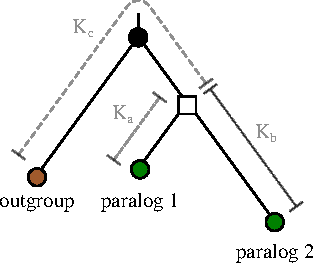
\includegraphics[width=0.4\columnwidth]{WGD_lengths.pdf}
	\end{center}
	\caption[Visualization of the asymmetry measures $R$ and $R'$]{Visualization of the quantities necessary to compute the asymmetry measures $R$ and $R'$. The WGD event is indicated by the square symbol ($\square$). The \textit{outgroup} is branching before the WGD.}
	\label{fig:wgd_lengths}
\end{figure}

\citet{byrne2007} analyzed 653 ohnolog
pairs in \textit{Saccharomyces cerevisiae}, \textit{Saccharomyces castellii} and \textit{Candida glabrata} that resulted from whole-genome duplication in a common ancestor of the three species. As outgroups, they used the corresponding orthologs in \textit{Kluyveromyces lactis}, a species that branched before the WGD event.

The resulting $R'$-values for the 188 ohnolog pairs in \textit{S. cerevisiae} are supplied by \citet{byrne2007}. Therefore, their distribution is used as a reference for modeling realistic substitution rate asymmetries. As by construction $R'>1$, a Gamma distribution with variable offset on the x-axis was fitted to the observed distribution. 

\begin{figure}[ht]
	\begin{center}     
		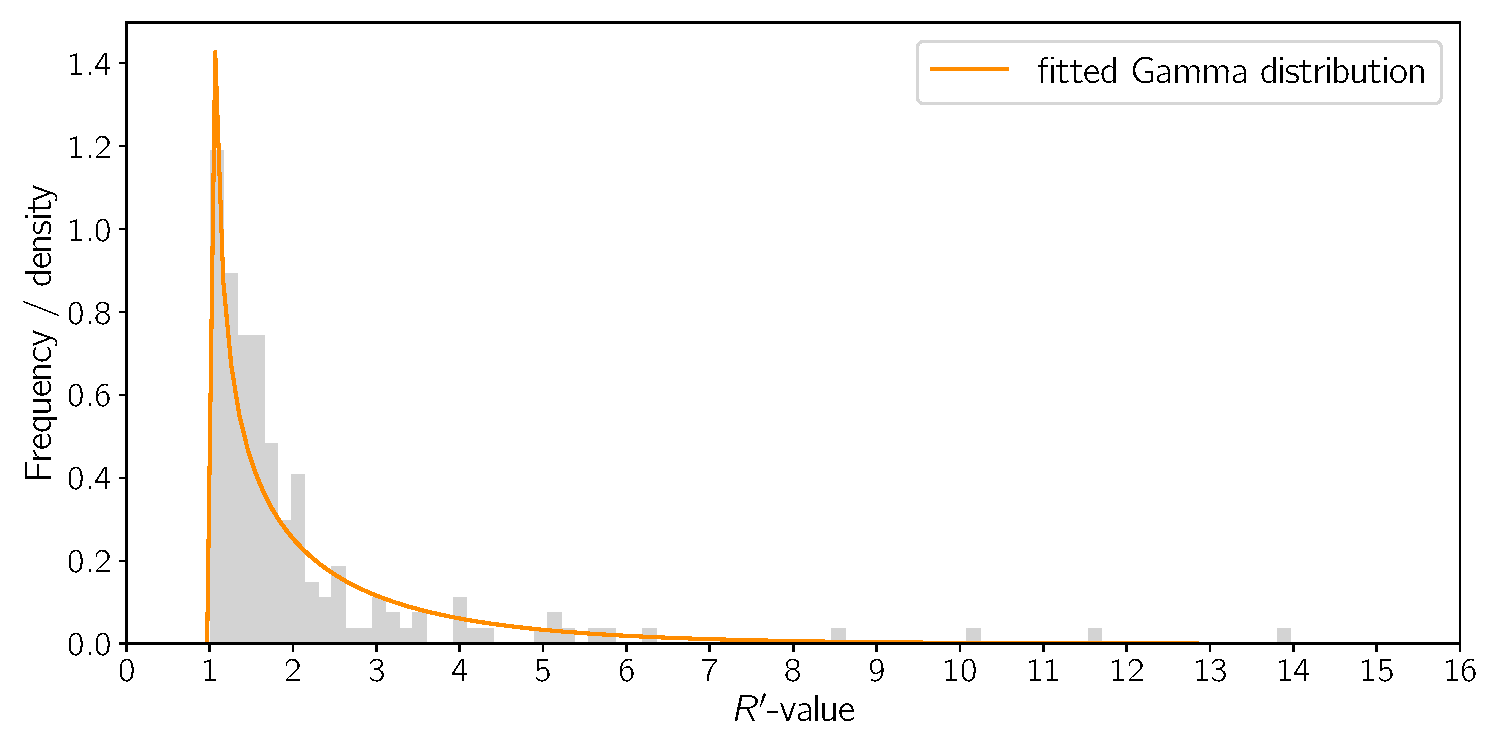
\includegraphics[width=\columnwidth]{WGD_histogram.pdf}
	\end{center}
	\caption[Histogram of $R'$-values measured for whole-genome duplication in \textit{S.~cerevisiae}]{Histogram of $R'$-values measured for whole-genome duplication in \textit{S.~cerevisiae} taken from \citet{byrne2007} and the probability density function of the fitted Gamma distribution (shape $k=0.538$, scale $\theta=2.183$, offset on x-axis $=1.007$). The $R'$-values are grouped into 80 equal-sized bins.}
	\label{fig:wgd_histogram}
\end{figure}

Both the histogram and the fitted Gamma distribution in Figure \ref{fig:wgd_histogram} show a concentration at lower asymmetries with a long tail on the right side indicating that large asymmetries like e.g.\ $R'=14$ are rare but possible. However, there are a couple of drawbacks arising from the choice of the data set. Firstly, duplicates resulting from a whole-genome duplication may behave differently than small-scale duplicates. It has been observed that the former are on average less divergent in sequence and functionality \citep{hakes2007}. The main reason being discussed for this is the effect of dosage advantages and disadvantages. In WGD, the genes of all components of protein complexes are copied resulting in the same relative amounts. In contrast, the imbalance of dosage after duplication of a single component is often deleterious. Whole-genome duplicates have been found to be enriched with such complex-building proteins which is in good accordance with this theory \citep{papp2003}. The higher selective pressure resulting from the maintenance of the interaction may thus be an explanation for the observations.

On the other hand, whole-genome duplicates all emerged at the same point in time, which is not true for small-scale duplicates and the independent development in separate branches of the species tree. This is especially problematic if the widely assumed theory holds that gene copies evolve fastest directly after the duplication and then slow down again \citep{jordan2004,innan2010}. In this case, the expected value of the $R'$ distribution should be highest directly after the degeneration and fate-determining phase and eventually slowly decrease again.

As a conclusion, data from small-scale duplications or perhaps a mixed data set should be preferred. The rate asymmetries after single-gene duplications have been investigated e.g.\ in rodents and show a magnitude comparable with the yeast data \citep{cusack2006,gayral2007}. However, data is available only for few duplicate pairs making the fitting of any theoretical distribution difficult. For this reason, the fitted Gamma distribution described above will be used here to model substitution rate imbalances. The procedure is explained in detail in Section~\ref{sec:imbalancing_implementation}.

\subsubsection{Substitution Rate Variance Among Species}
\label{sec:autocorrelation}

Another important source of substitution rate variance is the heterogeneity among the considered species. Mutation rates are negatively correlated with traits like body size and generation time and positively correlated with metabolic rate. Whilst the connection to generation time is explained intuitively by a slower establishment of mutations in the population, the latter is, e.g., linked to a higher abundance of aerobic respiration by-products and a generally increased DNA synthesis \citep{martin1993,gillooly2005,nabholz2007}.

As this also affects the singleton genes, i.e., genes having no paralogs in the same species, it constitutes an important aspect that violates the \emph{Molecular Clock Hypothesis} and should be taken into account for realistic evolution rate modeling.
The goal of this section is, therefore, to assign baseline rates for the conserved genes to all nodes and edges of the species tree.

\citet{kishino2001} simulate the development of the mutation rate $\varrho$ by sampling the rate of the ending node of an edge $uv$ from a log-normal distribution ($\textrm{Lognormal}(\mu,\sigma^2)$). To avoid bias towards increasing or decreasing rates, the mean~$\mu$ of the underlying normal distribution is normalized such that $\mathbf{E}(\varrho_v) = \varrho_u$. Since the expected value of a log-normal distribution is given by
\begin{equation}
\mathbf{E}(X) = e^{\mu + \frac{\sigma^2}{2}}
\end{equation}
the parameter $\mu$ must be set to 
\begin{equation}
\mu = \ln \varrho_u - \frac{\sigma^2}{2}
\end{equation}
to ensure this property. The divergence time of the edge, i.e., $\tau(u) - \tau(v)$ which is positive by construction, multiplied by a value $\sigma^2_0$ is used as variance parameter $\sigma^2$. Hence, the overall variance is given by
\begin{equation}
\begin{aligned}
\mathbf{Var}(\varrho_v) &= (e^{\sigma^2}-1)\, e^{2\mu+\sigma^2} \\
&= (e^{\sigma^2}-1)\, e^{2(\ln \varrho_u - \frac{\sigma^2}{2})+\sigma^2}\\
&= (e^{\sigma^2} - 1)\,\varrho_u^2\\
&= (e^{\sigma_0^2 (\tau(u)-\tau(v))} - 1)\,\varrho_u^2.
\end{aligned}
\end{equation}

Note that this method makes the implicit assumption that the temporal development of the mutation rate is a \emph{geometric Brownian motion} process, i.e., its logarithm follows a \emph{Brownian motion} (also called \emph{Wiener process}).
This can easily be seen by the fact that, for a \emph{geometric Brownian motion} process with random variable $X$ and an elapsed time $t$, the value of $X_t$ is also log-normally distributed \citep{oksendal1998}.
In particular, the expected value and variance are then given by 
\begin{equation}
\begin{aligned}
\mathbf{E}(X_t) &= X_0 e^{\mu t} \\
\mathbf{Var}(X_t) &= (e^{\sigma^2 t} -1)\, X_0^2 e^{2\mu t}.
\end{aligned}
\end{equation}
By setting $X_0=\varrho_u$ (the starting rate at vertex $u$), $\sigma^2=\sigma_0^2$ (the variable simulation parameter) and $\mu=0$ (in order to avoid bias towards in- or decreasing values) this becomes
\begin{equation}
\begin{aligned}
\mathbf{E}(\varrho_v) &= \varrho_u\\
\mathbf{Var}(\varrho_v) &= (e^{\sigma_0^2 (\tau(u)-\tau(v))} -1)\, \varrho_u^2
\end{aligned}
\end{equation}
for a specific edge $uv \in E(S)$, which is the same as above.

Having assigned rates to all vertices $v \in V(S)$ in a pre-order traversal, here, the effective rate $\varrho^0_e$ for an edge $e=uv \in E(S)$ is simply set to the arithmetic mean of its endpoints:
\begin{equation}
\varrho^0_e = \frac{\varrho_u + \varrho_v}{2}.
\end{equation}

As described in the next section, the rates $\varrho^0_e$ will be used as factors for the genes that are embedded into the respective edge of the species tree. This introduces a correlation between paralogs in the same species. Furthermore, the \emph{geometric Brownian motion} process generates a correlation between descending branches and their ancestors, referred to as \emph{autocorrelation} \citep{kishino2001}. The degree of autocorrelation is controlled by the factor $\sigma^2_0$. For an edge $uv \in E(S)$, a high value leads to a large variation of $\varrho_v$ w.r.t.\ the starting rate $\varrho_u$ and hence results in low autocorrelation. On the other hand, a low value of $\sigma^2_0$ indicates strong autocorrelation.


\subsubsection{Implementation}\label{sec:imbalancing_implementation}

As seen in the previous sections, several aspects have to be taken into account to simulate realistic substitution rate imbalances. Therefore, a hierarchical model is used that incorporates both the baseline rates $\varrho^0_e$ assigned to the branches of the species tree $S$ and the gene-specific effects resulting from unequal fates of gene copies after duplication and horizontal gene transfer events.

The values $\varrho^0_e$ for the edges $e=uv \in E(S)$ are determined by a pre-order traversal of $S$ as described in Section \ref{sec:autocorrelation}, where a user-defined mean substitution rate for the conserved members of the gene family is used as starting value $\varrho_{\rho_S}$ or $\varrho_{0_S}$ if the tree is planted, respectively.

For the contribution of asymmetric divergence of paralogs in an extended gene tree $T$, the following three types of duplication events are defined. Their relative occurrence is controlled by weights that can again be specified by the user:
\renewcommand{\labelenumi}{\roman{enumi})}
\begin{enumerate}
	\item \textit{Conservation}\\
	The child branches of such a duplication event will both be marked as\newline \texttt{conserved} (cf. positive dosage model).
	\item \textit{Subfunctionalization}\\
	The child branches of such a duplication event will both be marked as\newline \texttt{divergent} \citep[cf. DDC model by][]{force1999}.
	\item \textit{Neofunctionalization}\\
	One child branch will be marked as \texttt{conserved}, the other one as\newline \texttt{divergent} \citep[cf. neofunctionalization model by][]{ohno1970}.
\end{enumerate}

In the initialization phase, all vertices $u \in V(T)$ are sorted in natural temporal order, i.e., a node $v_1$ appears before $v_2$ in the list if $\tau(v_1) > \tau(v_2)$, where ties are broken arbitrarily. Furthermore, it is necessary to keep track of the current number of paralogous genes in each branch of the species tree during the simulation. As mentioned above, the edges of the gene tree $T$ can be marked as either \texttt{conserved} or \texttt{divergent} depending on the fate of the branch after a duplication event.

In order to record the gene-specific substitution rates $\varrho$, for each edge $e=uv \in E(T)$ an
empty list $\mathfrak{L}_e$ of ordered pairs of the form $(\tau,\varrho)$ is initialized, where $\varrho$ is a substitution rate and $\tau$ the corresponding time point at which the rate becomes valid during the existence of $e$. This especially enables the resetting of the gene status to \texttt{conserved} in
case it is the last survivor in a given species. At the moment, this is the main purpose of the introduction of the lists $\mathfrak{L}_e$. However, future extensions of the model can easily be adapted to consider other events that change the substitution rate during the existence of an edge. Moreover, temporarily restricted rate changes, as suggested by some duplication models \citep[cf.][]{innan2010}, are possible.
For easier notation, the i\textsuperscript{th} ordered pair $(\tau_i,\varrho_i)$ in $\mathfrak{L}_e$ is denoted by $\mathfrak{L}_{e,i}$. Furthermore, $\tau(\mathfrak{L}_{e,i}) \coloneqq \tau_i$ and
$\varrho(\mathfrak{L}_{e,i}) \coloneqq \varrho_i$.


Recall that $0_T\rho_T$ is the first (planted) edge in the gene tree $T$. The simulation is started by marking $0_T\rho_T$ as \texttt{conserved} and appending $(\tau(0_T), 1.0)$ to $\mathfrak{L}_{0_T\rho_T}$.
For each vertex $u$ in the sorted list, it then proceeds as follows:
\renewcommand{\labelenumi}{\alph{enumi})}
\renewcommand{\labelenumii}{\roman{enumii})}
\begin{enumerate}
	\item \textit{$u$ is a speciation event}\newline
	Mark all edges $uv$ with $v \in \child(u)$ the same as $\parent(u)u$. Append to $\mathfrak{L}_{uv}$the pair $(\tau(u), \varrho)$ with $\varrho=1.0$ ($uv$ is \texttt{conserved}) or $\varrho$ Gamma-distributed ($uv$ is \texttt{divergent}), respectively.
	\item \textit{$u$ is a duplication event}\newline
	If the edge $\parent(u)u$ is marked as \texttt{divergent}, then all edges $uv$ with $v \in \child(u)$ are also marked as \texttt{divergent} and corresponding pairs $(\tau(u),\varrho)$ are appended to
	$\mathfrak{L}_{uv}$, where the values of $\varrho$ are drawn i.i.d.\ from the Gamma distribution.
	If $\parent(u)u$ is marked as \texttt{conserved}, choose between 
	\begin{enumerate}
		\item conservation\newline
		mark both incident edges below $u$ as \texttt{conserved},
		\item subfunctionalization\newline
		mark both incident edges below $u$ as \texttt{divergent}, and
		\item neofunctionalization\newline
		mark one edge as \texttt{conserved} and the other as \texttt{divergent}
	\end{enumerate}
	with the specified weights.
	Append to $\mathfrak{L}_{uv}$ the pair $(\tau(u), \varrho)$ with $\varrho=1.0$ ($uv$ is \texttt{conserved}) or $\varrho$ Gamma-distributed ($uv$ is \texttt{divergent}), respectively.
	\item \textit{$u$ is a loss event}\newline
	If a single copy is left in the respective species after the loss: Let $e^*$ be the corresponding edge of the remaining copy at $\tau(u)$. Mark $e^*$ as \texttt{conserved} and append the pair $(\tau(u),1.0)$ to $\mathfrak{L}_{e^*}$.
	\item \textit{$u$ is an HGT event}\newline
	Let $v_1$ be the copy that remains in the species and $v_2$ the transferred copy. Mark $uv_1$ the same as $\parent(u)u$ and append $(\tau(u),\varrho)$ to $\mathfrak{L}_{uv_1}$ where $\varrho$ is the last rate that was appended to $\mathfrak{L}_{\parent(u)u}$. Mark $uv_2$ as \texttt{divergent} and append $(\tau(u),\varrho)$ to $\mathfrak{L}_{uv_2}$ with $\varrho$ Gamma-distributed.
\end{enumerate}

The simulation ends with the non-loss leaves of the gene. They belong to neither of the categories above, and, therefore, no further actions need to be performed. As a last step, for each edge $e=uv\in E(T)$, the list $\mathfrak{L}_{e}$ is finalized by appending $(\tau(v),\varrho)$ where $\varrho$ is the last rate that was appended to $\mathfrak{L}_{e}$ so far. This allows computing the edge length $\ell(e)$ for each edge $e$ in $T$ as a time-weighted mean of the assigned rates:
\begin{equation}
\ell(e) = \varrho_{f}^0
\sum_{i=1}^{|\mathfrak{L}_{e}|-1}\varrho(\mathfrak{L}_{e,i}) \cdot
(\tau(\mathfrak{L}_{e,i}) - \tau(\mathfrak{L}_{e,i+1}))
\end{equation}
where $f$ is the edge in the species tree $S$ into which $e$ is embedded.
The resulting distance function $\ell: E(T)\to \mathbb{R}^+$ induces an additive metric on the set of leaves $L(T)$ (see Section~\ref{sec:metrics}).

The following standard parameterization is used as default:

\begin{table}[H]
	\centering
	\setlength{\tabcolsep}{6pt}
	\renewcommand{\arraystretch}{1.7}
	\renewcommand\tabularxcolumn[1]{m{#1}}
	\begin{tabularx}{\textwidth}{ |m{5cm}|m{5cm}|Y|  }
		\hline
		\multicolumn{2}{|c|}{\textbf{Description}} & \textbf{Default value}\\
		\hline
		\multicolumn{2}{|l|}{mean substitution rate of the conserved genes} & 1.0 \\
		\hline
		\multicolumn{2}{|l|}{variance $\sigma_0^2$ for the baseline substitution rates in $S$} & 0.2 \\ 
		\hline
		\multirowcell{3}[1ex][l]{Gamma distribution\\for the (gene-specific)\\substitution rates $>1$\\ of divergent genes} & shape $k$ & 0.5 \\
		&scale $\theta$ & 2.2 \\
		&offset on the x-axis & 1.0 \\
		\hline
		\multirowcell{3}[1ex][l]{Duplication type\\weights} & conservation & $1/3$ \\
		&subfunctionalization & $1/3$ \\
		&neofunctionalization & $1/3$ \\
		\hline
	\end{tabularx}
	\caption{Default parameterization for the gene tree imbalancing used for the simulations. The parameters for the Gamma distribution were fitted to a yeast data set from \citet{byrne2007}, the rest is chosen arbitrarily.}
	\label{table:imbalancing_param}
\end{table}

To have the possibility to completely disable the asymmetric divergence after gene duplication, the \textit{conservation} mode was introduced. Among the models (see Table~\ref{table:dupl_models}), this scenario is best explained by those that assume an advantageous dosage effect, in which the function is kept for both copies and the selective pressure is the same for both (possibly slightly relaxed).

The question which of the two theoretic models neofunctionalization and subfunctionalization occurs more often in biologic systems has been addressed in several studies. Therein, the comparison of gene expression profiles in different tissues was used as a proxy to decide for an individual pair of paralogs which of the scenarios is more likely \citep{lien2016,braasch2016}. In this framework, a partitioning of expression regulation indicates subfunctionalization, and, e.g., the expression in a new tissue w.r.t.\ a related species that branched before the duplication event is characteristic for neofunctionalization. Whilst \citet{lien2016} found that neofunctionalization is most abundant in teleosts, \citet{braasch2016} found more evidence for a dominance of subfunctionalization (also in fish expression data). However, a reanalysis of the data by \citet{sandve2018} showed that these discrepancies are a result of the different methods and interpretation in the two studies. As it is hard to come by reliable numbers that can be used as weights for the choice between duplication event types, here, an \textit{a priori} uniform distribution is assumed for the three modes \textit{conservation}, \textit{subfunctionalization} and \textit{neofunctionalization}. The weights $w_C=w_S=w_N=1/3$ are thus used as the default setting.

Another possible approach to handle this issue would be to use a prior distribution for the weighting and choose them randomly for an individual gene tree. The same could be applied for parameters like the mean substitution rate of the conserved members of the gene family and the variance factor $\sigma^2_0$. The current implementation could easily be extended with such priors in future refinements.

\subsection{Simulated Measurement Noise}
\label{sec:measurement_noise}

A simulated gene tree $T$ with weight function $\ell: E(T)\to \mathbb{R}^+$, as described so far, induces an additive metric on the set of its leaves. For evaluating the performance of phylogenetic reconstruction algorithms, the distances between the non-loss leaves, i.e., the extant genes at time $\tau=0$, are of special interest, since they represent the measurable part of the metric in real data.

The number of mutation events that occurred on the path between two genes is not directly observable, in particular, due to backmutations. As a consequence, simple dissimilarity measures like the Hamming distance in pairwise alignments are not additive. This issue can partly be overcome by applying a distance correction with a suitable model for DNA evolution \citep{jukes1969,kimura1980,tavare1986}.
Such transformations yield good approximations to the true evolutionary distances in most cases, but all models make assumptions for the sequence evolution that might not be realistic. Moreover, they must rely on the quality of the alignment. Hence, both steps can introduce noise and bias into the data.

Another important aspect, that was already mentioned, is that both nucleic acid and protein sequences have a limited length. As the approximation of distances relies on the quantification of discrete evolutionary events, they are difficult to estimate for very short sequences. Also, the DNA evolution models often produce poor results in case the alignment is saturated, i.e., most base or amino acid positions have undergone mutations and backmutations \citep{philippe2011}.

As a consequence, it is necessary to introduce measurement noise to produce realistic test data for any phylogenetic and orthology detection tool. Two approaches for noise simulation have been implemented: random perturbations drawn from a normal distribution and a systematic disturbance with a wrong tree topology.

\subsubsection{Random Perturbations}

The first strategy for the introduction of measurement noise aims to avoid a systematical bias. Therefore, random perturbations $\epsilon_{xy}$ are drawn from a normal distribution with mean 1 and a user-defined standard deviation $\sigma$. The noise is then incorporated into the distance matrix $\mathbf{D}$ (on the leaf set $L$ of a gene tree $T$) by substituting
$\mathbf{D'}(x,y)=\mathbf{D'}(y,x)= \varepsilon_{xy}\mathbf{D}(x,y)$. Note that using multiplicative noise with mean~1 avoids that small distances `suffer' more from bigger (absolute) perturbations than large distances, as it would be the case for additive noise with mean~0.

Most phylogenetic inference methods rely on additive metric data \citep[cf.][]{retzlaff2018}. In general, the introduction of noise does not preserve this property, especially by violating the triangle inequality. Whilst additivity is hard to be guaranteed, Algorithm \ref{alg:noise_unbiased} is applied to ensure that the disturbed matrix $\mathbf{D'}$ is still a metric.

\begin{algorithm}[ht]
	\caption{Introduction of random measurement noise into $\mathbf{D}$}
	\label{alg:noise_unbiased}
	\SetAlgoLined
	\DontPrintSemicolon
	\Input Additive distance matrix $\mathbf{D}$ with dimension $|L| \times |L|$, standard deviation $\sigma$ \;
	\Output Disturbed matrix $\mathbf{D}'$ \;
	Initialize $\mathbf{D'} = \mathbf{D}$.\;
	Initialize $n_{\textrm{success}} = 0$.\;
	\While{$n_{success} < \binom{|L|}{2}$}{
		Draw $x \ne y \in L$ randomly.\;
		Draw $\varepsilon_{xy}$ from $\mathcal{N}(1,\sigma^2) $.\;
		Set $d_{\textrm{old}} = \mathbf{D'}(x,y)$.\;
		Set $\mathbf{D'}(x,y)=\mathbf{D'}(y,x) \leftarrow \varepsilon_{xy}\mathbf{D}'(x,y)$.\;
		\uIf{$ \mathbf{D'} $ is a metric\;}{
			$n_{\textrm{success}} \leftarrow n_{\textrm{success}} + 1$\;
		}
		\Else{Set $\mathbf{D'}(x,y)=\mathbf{D'}(y,x) \leftarrow d_{\textrm{old}}$.\;
		}
	}
\end{algorithm}

The idea of this algorithm is to simply reject all perturbations that violate the triangle inequality. The process is repeated until $\binom{|L|}{2}$ changes have been accepted to ensure an appropriate scaling with the size of the input matrix. Note that not all cell entries will be changed in most cases, whereas some are changed multiple times. In every iteration step, $\mathcal{O}(|L|)$ inequalities have to be checked. For moderate noise, the number of iterations should not exceed $\mathcal{O}(|L|^2)$. Hence, the time complexity of the procedure is at least $\mathcal{O}(|L|^3)$. This approach will be referred to as \emph{Rejection method} in the following.

In an alternative strategy, noise is first added to the distance of every unordered pair $x \ne y \in L$. In a subsequent step, the disturbed matrix is then modified such that it is again a metric. This task is known as the \textit{metric repair} or \textit{metric nearness problem} for which several algorithms have been suggested \citep[e.g. cf.][]{brickell2008,gilbert2017}. To this end, random perturbations drawn from a normal distribution with mean 1 and standard deviation $\sigma$ are multiplied to each of the $\binom{|L|}{2}$ distinct distances between the leaves $x \ne y \in L$. In the case of negative values, a new disturbance is drawn. In a subsequent step, one of the algorithms for \textit{sparse metric repair} described by \citet{gilbert2017} is applied to extract a distance matrix from the disturbed data that again satisfies the properties of a metric.

The first metric repair algorithm that was implemented here is the \textit{Decrease Only Metric Repair (DOMR)} in which a perturbation matrix $\mathbf{P}$ is searched such that $\mathbf{\hat{D}}=\mathbf{D'}+\mathbf{P}$ is a metric and the values in $\mathbf{D'}$ are only decreased. A modified Floyd-Warshall algorithm is used to ensure that $\mathbf{\hat{D}}$ is a metric and that $\mathbf{P}$ is minimal w.r.t.\ the $\ell_1$ norm. The second algorithm is a heuristic for a \textit{General Metric Repair (GMR)}, i.e., there are no restrictions for the matrix $\mathbf{P}$. In contrast to \emph{DOMR}, this approach does not guarantee the resulting matrix to be a metric.

The \textit{Rejection method} seems to produce the most stable results and is therefore used as default.

\subsubsection{Wrong Topology Bias}
\label{sec:wrong_topology_noise}

The correct topology of a phylogenetic tree can be inferred from additive metric distance data with the exception of the location of the root \citep[][]{bandelt1986,saitou1987}. It is therefore of interest to examine the sensitivity to systematic disturbances for tools that explicitly make use of topology reconstruction.

To this end, small contributions of a second distance matrix $\mathbf{D}^*$ of equal dimension are added to $\mathbf{D}$ by forming a convex linear combination:
\begin{equation}
\mathbf{D'} = (1-\alpha)\mathbf{D} + \alpha \mathbf{D}^* \qquad 0\le \alpha\le 1.
\end{equation}
If both $\mathbf{D}$ and $\mathbf{D}^*$ are metrics, the resulting matrix $\mathbf{D'}$ will also be a metric. The first three properties of metrics are trivially preserved. It can also easily be seen that no triangle is destroyed by considering that multiplying inequalities with a factor greater than zero and adding them preserves the inequality.

For a specific scenario with species tree $S$ and an observable gene tree $T$ giving rise to the distance matrix $\mathbf{D}$, the disturbance matrix $\mathbf{D}^*$ is constructed as follows: A second gene tree $T_2$ is simulated along $S$ and a corresponding distance matrix $\mathbf{D}_2$ is computed. If $|L(T)| \le |L(T_2)|$, the upper left corner of $\mathbf{D}_2$ is simply used as $\mathbf{D}^*$. Otherwise, $\mathbf{D}_2$ is recycled by placing it in multiple rows and columns until the dimension of $\mathbf{D}$ is filled where overhanging cells are cut off. 


\bibliographystyle{plainnatnourl}
\bibliography{references}


\section*{Notation}
\addcontentsline{toc}{chapter}{Notation}

\vspace{5mm}
{\renewcommand{\baselinestretch}{1.12}\footnotesize
	\begin{minipage}[t]{0.47\textwidth}
		\textbf{Graphs}
		
		\vspace{2mm}
		\noindent
		$G=(V,E)$ -- undirected graph\\
		$V$ -- set of vertices\\
		$E$ -- set of edges\\
		$\G$ -- directed graph\\
		$x,y$ -- vertices\\
		$e,f$ -- edges\\
		$xy$ -- undirected edge between x and y\\
		$(x,y)$ -- directed edge between x and y\\
		$P$ -- path\\
		$\degree(x)$ -- degree of vertex $x$\\
		$\mathcal{C}$ -- set of connected components\\
		
		\noindent
		\textbf{(Phylogenetic) Trees}
		
		\vspace{2mm}
		\noindent
		$T=(V,E)$ -- rooted (gene) tree\\
		$T_{\textrm{obs}}$ -- observable gene tree\\
		$\unrooted{T}$ -- unrooted (gene) tree\\
		$S$ -- species tree\\
		$0_T, 0_S$ -- planted root\\
		$\rho_T, \rho_S$ -- root (first branching event)\\
		$u,v,w$ -- vertices\\
		$l, x, y, z$ -- genes / leaves\\
		$r, s, s_1, s_2$ -- species\\
		$\parent(v)$ -- parent of $v$\\
		$\child(v)$ -- set of children of $v$\\
		$V^0(T)$ -- inner vertices\\
		$L(T)$ -- leaves\\	
		$L[s]$ -- leaves of color/species $s$\\
		$T(v)$ -- subtree rooted at $v$\\
		$\preceq_T$ -- ancestor relation\\
		$\lca_T(A)$ -- last common ancestor of set $A$\\
		$xy|z$ -- rooted triple\\
		$(xy|uv)$ -- quartet relation\\
		$\sigma(x)$ -- leaf coloring map\\
		$\mu(v)$ -- reconciliation map\\
		$\tau(v)$ -- dating function\\
		$d_{\tau}(x,y)$ -- divergence time\\
		$\ell(e)$ -- length of edge $e$\\
		$d(x,y)$ -- (evolutionary) distance\\
		
		\noindent
		\textbf{Event labeling}
		
		\vspace{2mm}
		\noindent
		$t(v)$ -- event labeling map\\
		$\ROOT$ -- (planted) root\\
		$\LEAF$ -- leaf\\
		$\SPEC$ -- speciation\\
		$\DUPL$ -- duplication\\
	\end{minipage}
	\hfill
	\begin{minipage}[t]{0.47\textwidth}
		$\HGT$ -- horizontal gene transfer (HGT)\\
		$\dashv$/$*$ -- loss\\
		
		\noindent
		\textbf{Orthology and Best Matches}
		
		\vspace{2mm}
		\noindent
		$\Theta$ -- (true) orthology graph\\
		$\unrooted{\Theta}$ -- (true) paralogy graph\\
		$\G$ -- colored Best Match Graph (cBMG)\\
		$G$ -- colored Reciprocal Best Match Graph (cRBMG)\\
		$x \rightarrow y$ -- best match relation\\
		$\left< a_1bca_2\right>$ -- induced $P_4$\\
		
		\noindent
		\textbf{Inference methods}
		
		\vspace{2mm}
		\noindent
		$\mathbf{D}$ -- distance matrix\\
		$\epsilon$ -- relative tolerance threshold\\
		$\eta$ -- discarding threshold for outgroup species\\
		$\mathscr{R}$ -- triple set\\
		$\mathscr{L}$ -- leaf set\\
		$\mathscr{H}$ -- auxiliary graph (\texttt{BUILD})\\
		$L_e$ -- leaf set (extant genes)\\
		$L_0$ -- leaf set (losses)\\
		$Z_v$ -- set of outgroups for vertex $v\in V(S)$\\
		
		\noindent
		\textbf{Simulation}
		
		\vspace{2mm}
		\noindent
		$d, l, h$ -- event rates\\
		$g\in G(\tau)$ -- extant gene at time $\tau$\\
		$q\in Q$ -- event type\\
		$\xi=(g,q)$ -- `reaction' in Gillespie algorithm\\
		$r_{\xi}(\tau)$ -- rate of reaction $\xi$\\
		$R(\tau)$ -- total rate\\
		$\Delta\tau$ -- waiting time\\
		$\mathcal{P}$ -- priority queue\\
		$K_A$ -- non-synonymous substitution rate\\
		$K_S$ -- synonymous substitution rate\\
		$\omega$ -- measure for selection pressure\\
		$R,R'$ -- asymmetry measures\\
		$\varrho$ -- evolution rate\\
		$k, \theta$ -- shape and scale (Gamma distribution)\\
		$\mathfrak{L}_e$ -- list of assigned rates to edge $e$\\
		$w_C, w_N, w_S$ -- weights for duplication types\\
		$\sigma$ -- standard deviation (normal distribution)\\
		$\alpha$ -- contribution of the disturbance matrix in a convex combination\\
		$\mathbf{D'}$ -- disturbed distance matrix\\
		
	\end{minipage}
	
}

\end{document}
